\documentclass[10pt,spanish,a4paper,notitlepage]{article}
\usepackage[spanish,es-tabla]{babel}  	% Traduce los textos a castellano
\usepackage[utf8]{inputenc}
\usepackage{units}
\usepackage{fancyhdr}
\usepackage{anysize}
\usepackage{float}
\usepackage[dvipsnames]{xcolor}
\usepackage{abstract} % paquete para el resumen del articulo
\usepackage[square,sort,comma,numbers]{natbib}
\usepackage{graphicx}
\usepackage{tablefootnote} % para agregar notas al pie de pagina en las tablas
\usepackage{amsmath} % para agregar acentos a las variables matemáticas, como por ej ^ para indicar el valor pico
\usepackage{hyperref} % para agregar url
\usepackage[bottom]{footmisc} % para que las footnote estén al final de la hoja y no cuando termina el texto
\usepackage{multirow}
\usepackage{amssymb}
\usepackage{subcaption}

\usepackage[europeanvoltages]{circuitikz}

\setcitestyle{square} %cambio las citas a [] en lugar de ()

% todo lo que sigue es para poner links que se les pueda hacer click
\usepackage{xcolor}
\usepackage[normalem]{ulem}
\usepackage{hyperref}
\hypersetup{colorlinks,urlcolor=blue}


\setlength{\headheight}{33pt} 

\makeatletter
\DeclareUrlCommand\ULurl@@{%
  \def\UrlFont{\ttfamily\color{blue}}%
  \def\UrlLeft{\uline\bgroup}%
  \def\UrlRight{\egroup}}
\def\ULurl@#1{\hyper@linkurl{\ULurl@@{#1}}{#1}}
\DeclareRobustCommand*\ULurl{\hyper@normalise\ULurl@}
\makeatother

%---------------------------------------Configuraciones de pagina----------------------------------------------
\marginsize{2.5cm}{2.5cm}{1cm}{1cm}

\pagestyle{fancy}
\fancyhf{}
\lhead{
86.06 - \textsc{Circuitos Electrónicos}\\ 
1\textsuperscript{er} Cuatrimestre de 2016
}
\rhead{
\includegraphics[width=3cm]{includes/FIUBA_ALTA.jpg}}
\rfoot{Página \thepage}

%------------------------------ graphicx ----------------------------------
%
% Todas las imagenes estan en el directorio tp-img:
%
\newcommand{\imgdir}{includes}
\graphicspath{{\imgdir/}}
%


%------------------------- Inicio del documento ---------------------------

\begin{document}

\begin{titlepage}

\thispagestyle{empty}

\begin{center}

\includegraphics[width=5cm]{fiuba}\\
\large{\textsc{Universidad de Buenos Aires}}\\
\large{\textsc{Facultad De Ingeniera}}\\
\small{2016 - 1\textsuperscript{er} Cuatrimestre}
\end{center}

\vfill
\begin{center}
\Large{\underline{86.06 - \textsc{Circuitos Electrónicos}}}
\end{center}

\vfill

\begin{tabbing}
\hspace{2cm}\=\+TRABAJO DE LABORATORIO 3\\
	Etapas con transistores integrados\\
	\today\\
\\
	INTEGRANTES:\hspace{-1cm}\=\+\hspace{1cm}\=\hspace{6cm}\=\\
		Bruno, Nicolas	\>\> 95191\\
			\>\footnotesize{$<$nicoo.24@hotmail.com$>$}\\
		Piñero, Juan Cruz	\>\> 96112\\
			\>\footnotesize{$<$juan.cruzp@yahoo.com$>$}\\
		Vazquez, Matias	\>\> 91523\\
			\>\footnotesize{$<$mfvazquezfiuba@gmail.com$>$}\\
\end{tabbing}

\vfill

\hrule
\vspace{0.2cm}

\end{titlepage}

%
% Hago que las paginas se comiencen a contar a partir de aqui
%
\setcounter{page}{1}

%
% Pongo el indice en una pagina aparte:
%
\tableofcontents
\newpage

\section{Introducción}

En el siguiente trabajo se analizaran las características de una etapa amplificadora formada por dos transistores de tecnología metal-oxido-semiconductor (MOSFET), en configuración ``cascode'' (Source común - Gate común). Para esto, se realizará en un primer lugar el calculo analítico, para luego contrastarlo con la simulación y la medición.

\section{Cálculo analítico}

El circuito a analizar es el de la figura \ref{fig:circuitototal}. Se consideran despreciables $\lambda$ y $\gamma$ ($\lambda = 0$ y $\gamma = 0$). Las ecuaciones que describen a cada transistor son las siguientes:

\begin{equation}
     V_T=V_{T0}+\gamma \left( \sqrt{ | V_{SB}+2\phi_{F} | } - \sqrt{|2\phi_{F}|} \right)
    \label{eq:VT}
\end{equation}

\begin{equation}
    I_D={k}' \frac{W}{L} \left ( V_{GS}-V_{T} \right )^{^{2}}
    \label{eq:ID}
\end{equation}

Donde ${k}'=\frac{k_p}{2}$. De la ecuación \ref{eq:VT} se tiene que la tensión umbral de ambos transistores será $V_{T0}$ ya que se despreció el parámetro $\gamma$. Por lo tanto se tienen los siguientes parámetros:

\begin{itemize}
\item ${k_1}'=7.5\unit{\frac{mA}{V^2}}$
\item ${k_2}'=100\unit{\frac{mA}{V^2}}$
\item ${V_{T1}}'= -1\,\unit{V}$
\item ${V_{T2}}'= -1\,\unit{V}$
\item $\frac{W}{L}=1$ (para ambos transistores)
\end{itemize}

\begin{figure}[H]
\centering
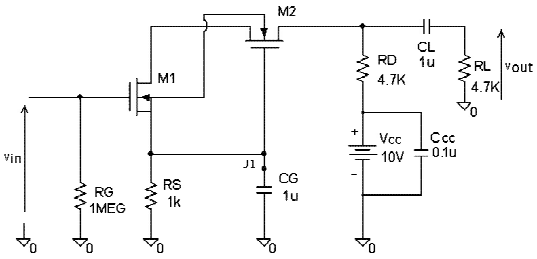
\includegraphics[scale=1]{circuitos/circuitototal.png}
\caption{Circuito a analizar}
\label{fig:circuitototal}
\end{figure}


\subsection{Punto de reposo}

Para el cálculo analítico del punto de reposo, se analiza el circuito de polarización del circuito de la figura \ref{fig:circuitototal}. El mismo puede observarse en la figura \ref{fig:circuitoreposo}.

\begin{figure}[H]
\centering
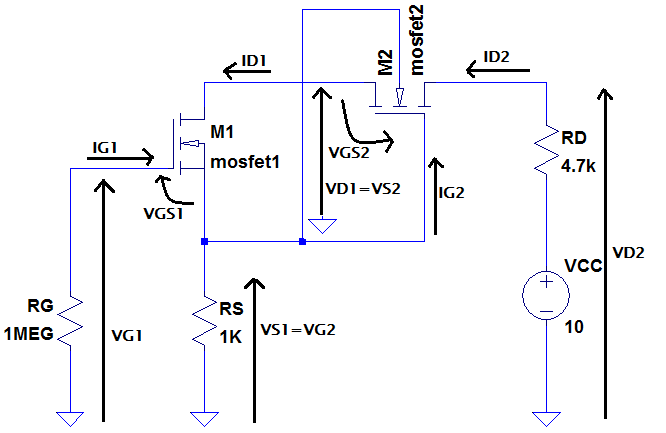
\includegraphics[scale=0.8]{circuitos/reposoanalitico.png}
\caption{Circuito para calcular el punto de reposo}
\label{fig:circuitoreposo}
\end{figure}

Debido a considerar que la impedancia de entrada de los MOSFET es infinita, se tiene que $I_{G1}=I_{G2}=0$. También se tiene que $I_{B2}=0$. Por lo tanto $I_{D1}=I_{D2}=I_D$. Recorriendo la malla de entrada del primer transistor, se tiene que:

\begin{equation}
    V_{GS1}=-I_D 1\,\unit{k\Omega}
    \label{eq:vgs1}
\end{equation}

Reemplazando \ref{eq:vgs1} en \ref{eq:ID} (con los datos para el primer transistor) se obtiene que $I_D=0.7\,\unit{mA}$. Usando este corriente en \ref{eq:vgs1} se obtiene que $V_{GS1}=-0.7\,\unit{V}$. Luego, debido a que las corrientes de drain son iguales, utilizando nuevamente la ecuación \ref{eq:ID} pero con los datos para el transistor segundo transistor se obtiene que $V_{GS2}=-0.92\,\unit{V}$. 

\begin{equation}
    V_{S1}=-I_D 1\,\unit{k\Omega}
    \label{eq:vs1}
\end{equation}

De \ref{eq:vs1}, utilizando la corriente calculada anteriormente, se obtiene que $V_{S1}=0.7\,\unit{V}$. Observando el circuito se ve que $V_{S1}=V_{G2}=V_{B2}$, por lo tanto 

\begin{equation}
    V_{S2}=V_{G2}-V_{GS2}
    \label{eq:vs2}
\end{equation}

De lo que se obtiene que $V_{S2}=1.62\,\unit{V}$. Para el calculo de la tensión de drain del segundo transistor se tiene que:

\begin{equation}
    V_{D2}= 10\,\unit{V}-I_D 4.7\,\unit{k\Omega}
    \label{eq:vd2}
\end{equation}

Resolviendo, $V_{D2}=6.71\,\unit{V}$. También se tiene que $V_{S2}=V_{D1}$, por lo tanto $V_{D1}=1.62\,\unit{V}$. En la tabla \ref{table:valoresreposo} pueden verse las tensiones contra común, y las corrientes en reposo. También se agregan las tensiones gate-source drain-source para mostrar que los transistores se encuentran en régimen lineal.


\begin{table}[H]
\centering
\begin{tabular}{|c|c|c|c|c|c|c|} 
\hline
Transistor & $V_{G}$ & $V_{S}$ & $V_{D}$ & $I_{D}$ & $V_{GS}$ & $V_{DS}$  \\ \hline
M1 & $0\,\unit{V}$ & $0.7\,\unit{V}$  & $1.62\,\unit{V}$ & $0.7\,\unit{mA}$ & $-0.7\,\unit{V}$  & $0.92\,\unit{V}$ \\ \hline
M2 & $0.7\,\unit{V}$ & $1.62\,\unit{V}$ & $6.71\,\unit{V}$ & $0.7\,\unit{mA}$ & $-0.92\,\unit{V}$ & $5.09\,\unit{V}$\\ \hline
\end{tabular}
\caption{Corrientes y tensiones contra común en reposo}
\label{table:valoresreposo}
\end{table}


\subsection{Amplificación de tensión total (\texorpdfstring{$A_v$}{TEXT}) a frecuencias medias}

Para realizar este cálculo analítico se analiza el circuito de señal (ver figura \ref{fig:senalanalitico})

\begin{figure}[H]
\centering
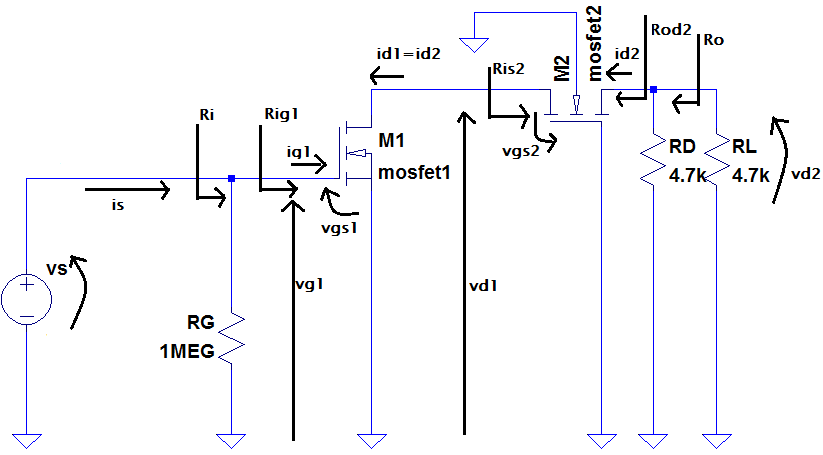
\includegraphics[scale=0.7]{circuitos/senalanalitico.png}
\caption{Circuito para calcular la ganancia $A_v$ a freucencias medis}
\label{fig:senalanalitico}
\end{figure}

En primer lugar se calcula el parámetro gm utilizando la formula \ref{eq:gm}, de lo que se obtiene ${g_{m1}}=4.6\unit{\frac{mA}{V}}$ y ${g_{m2}}=17\unit{\frac{mA}{V}}$

\begin{equation}
     g_m=2\sqrt{k' \frac{W}{L} I_{DQ}}
    \label{eq:gm}
\end{equation}

Para calcular la ganancia de la primera etapa es necesario conocer su carga, para esto se calcula por inspección la resistencia de entrada de la segunda etapa. Para obtener esta resistencia, se conecta una fuente de prueba en el terminal de source de la segunda etapa como se indica en la figura \ref{fig:Ris2}. Por lo tanto la resistencia se obtiene como indica la ecuación \ref{eq:Ris22}.


\begin{figure}[H]
\centering
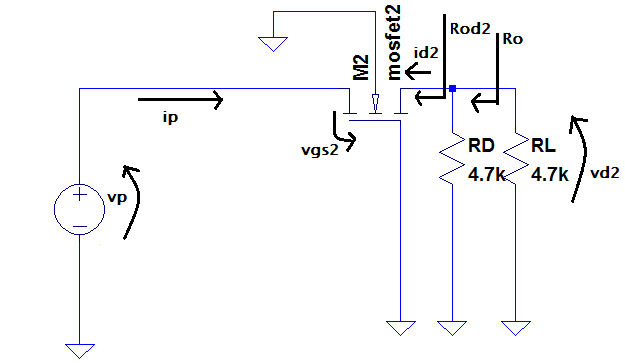
\includegraphics[scale=0.7]{circuitos/Ris2.png}
\caption{Circuito para calcular la resistencia $R_{is2}$}
\label{fig:Ris2}
\end{figure}

\begin{equation}
     R_{is2}= \frac{v_p}{i_p}= \frac{r_{gs}}{\beta_{FET}}=\frac{1}{g_{m2}}= 59\,\unit{\Omega}
     \label{eq:Ris22}
\end{equation}

Por lo tanto la ganancia de la primera etapa se calcula como se indica en la ecuación \ref{eq:Av1}.

\begin{equation}
     A_{v1}=\frac{v_{d1}}{v_{g1}}=\frac{-i_{d1}R_{is2}}{v_{gs1}}=\frac{-g_{m1}v_{gs1}R_{is2}}{v_{gs1}}=-g_{m1}R_{is2}=-0.27
     \label{eq:Av1}
\end{equation}

Se calcula la ganancia de la segunda etapa con la ecuación \ref{eq:Av2}

\begin{equation}
     A_{v2}=\frac{v_{d2}}{v_{d1}}=\frac{-i_{d2}(R_{D}//R_{L})}{v_{gs2}}=\frac{g_{m2}v_{gs2}(R_{D}//R_{L})}{v_{gs2}}=g_{m2}(R_{D}//R_{L})=40
     \label{eq:Av2}
\end{equation}

Por lo tanto la ganancia total se calcula como indica la ecuación \ref{eq:Avtotal}

\begin{equation}
     A_{v}=\frac{v_{d2}}{v_{g1}}=\frac{v_{d2}}{v_{d1}} \frac{v_{d1}}{v_{g1}}= A_{v1}A_{v2}=-10.8
     \label{eq:Avtotal}
\end{equation}

\subsection{Resistencia de entrada y de salida}

\subsubsection{Resistencia de entrada \texorpdfstring{$R_i$}{TEXT}}

El cálculo de la resistencia de entrada es trivial debido a que se 
considera  infinita la impedancia de entrada del MOSFET. Se calcula
$R_i$ mediante la ecuación \ref{eq:Ri}:

\begin{equation}
    R_{i}=R_G//R_{ig1} \approx R_G=1\,\unit{M\Omega}
    \label{eq:Ri}
\end{equation}

\subsubsection{Resistencia de salida \texorpdfstring{$R_o$}{TEXT}}

Para el cálculo de $R_o$ se considera que la resistencia de salida de la primer etapa
tiende a infinito, ya que es $r_{ds1}$. Por lo que se considerará $i_{s2} = 0$.
Bajo estas condiciones se obtiene que $R_{od2} = \beta_{FET} r_{ds2}$ y como
se considera que $r_{ds2}$ tiende a infinito, $R_{od2}$ tenderá a infinito.

Por lo que $R_o$ se calcula según la ecuación \ref{eq:Ro}.

\begin{equation}
    R_o = R_D // R_{od2} \approx R_D = 4.7\,\unit{k\Omega}
    \label{eq:Ro}
\end{equation}

\subsection{Excursión de salida}

\subsubsection{Máxima excursión de salida sin recorte}

Se obtendrá la máxima excursión de cada etapa para luego poder obtener
la total.\\

\begin{itemize}
\item \textbf{Primer Etapa}\\

Se obtienen los valores pico de la tensión de salida de la primer etapa $\overset{\wedge}{v_{d1}}$
en los cuales el transistor entra en la región de corte o triodo. 
Para que el transistor esté en triodo debe cumplirse que:

\[ \displaystyle \widehat{v_{d1_{triodo}}} = V_{DS1Q} = 0.92\,\unit{V} \]


Para que el transistor esté en la región de corte, debe cumplirse que $i_{D1} = 0\,\unit{A}$.

Como:

\[ \displaystyle  i_{D1} = I_{D1Q} + i_{d1} \]

Entonces:

\[ \displaystyle i_{d1_{corte}} = i_{D1} - I_{D1Q} = 0\,\unit{mA} - 0.7\,\unit{mA} = -0.7\,\unit{mA} \]

Y por lo tanto:

\[ \displaystyle \widehat{v_{d1_{corte}}} = |i_{d1_{corte}} R_{is2}| = 0.7\,\unit{mA}\ 59\,\unit{\Omega} = 41.3\,\unit{mV} \]

Como $\widehat{v_{d1_{corte}}} < \widehat{v_{d1_{triodo}}}$ la excursión
máxima de salida sin recorte de la primer etapa será:

\begin{equation}
\widehat{v_{d1}} = \widehat{v_{d1_{corte}}} = 41.3\,\unit{mV}
\label{eq:vd1_max}
\end{equation}

\item \textbf{Segunda etapa}\\

Para la segunda etapa se considerará que $v_o \approx v_{ds2}$ ya que
$v_{gs2} \approx 0\,\unit{V}$.
Entonces el transistor entrará en la región de triodo cuando:

\[ \displaystyle \widehat{v_{o_{triodo}}} = V_{DS2Q} = 5.09\,\unit{V} \]

Y entrará en la región de corte cuando $i_{D2} = 0\,\unit{A}$.

Entonces:

\[ \displaystyle i_{d2_{corte}} = i_{D2} - I_{D2Q} = -0.7\,\unit{mA} \]

Por lo tanto:

\[ \displaystyle \widehat{v_{o_{corte}}} = |i_{d2_{corte}} R_{da}| = 0.7\,\unit{mA}\ 2.35\,\unit{k\Omega} = 1.65\,\unit{V} \]

Como $\widehat{v_{o_{corte}}} < \widehat{v_{o_{triodo}}}$ la excursión
máxima de salida sin recorte de la segunda etapa será:

\begin{equation}
\widehat{v_{o}} = \widehat{v_{o_{corte}}} = 1.65\,\unit{V}
\label{eq:vo_max}
\end{equation}

\end{itemize}

Ahora se verificará si para $\widehat{v_{o}}$ no hay recorte en la primer etapa.
Si $v_o = 1.65\,\unit{V}$ entonces:

\[ \displaystyle v_{d1} = \frac{v_o}{A_{v2}} = \frac{1.65\,\unit{V}}{40} = 41.3 \,\unit{mV}\]

Este resultado es igual a la máxima excursión de salida sin recorte de la primer etapa. Por lo tanto, si no hay recorte en la segunda etapa, no habrá recorte en 
la primer etapa.

Finalmente la máxima excursión de salida sin recorte es:

\[ \displaystyle \widehat{v_o} = 1.65\,\unit{V} \]

Por lo que el valor máximo de la señal de entrada $v_i$ es:

\[ \displaystyle \widehat{v_i} = \left| \frac{v_o}{A_{v}} \right| = \left| \frac{1.65\,\unit{V}}{10.8} \right| = 153 \,\unit{mV} \]

\subsubsection{Máxima excursión de salida sin distorsión}

Se estima que existe baja distorsión cuando $\Delta V_{GS} << V_{GS0} - V_T$. Siendo $V_{GS0}$ el valor de $V_{GS}$ en el cual la recta
tangente al punto Q de la curva $I_D(V_{GS})$ tiene $I_D = 0\,\unit{A}$. Como se muestra en la figura \ref{fig:curva_distorsion}.

\begin{figure}[H]
\centering
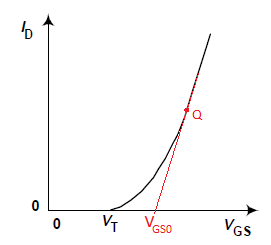
\includegraphics[scale=0.8]{curvas/distorsion_curva.png}
\caption{Curva $V_{GS}$ vs $I_D$ del transistor}
\label{fig:curva_distorsion}
\end{figure}

Para obtener $V_{GS0}$ se plantea la ecuación de la recta tangente:

\[ \displaystyle I_D = I_{DQ} + 2k'\frac{W}{L} (V_{GSQ} - V_T) (V_{GS} - V_{GSQ}) \]

Luego se despeja $V_{GS}$ cuando $I_D = 0\,\unit{A}$:

\[ \displaystyle V_{GS0} = V_{GSQ} - \frac{I_{DQ}}{2k'\frac{W}{L} (V_{GSQ} - V_T)} \]

Luego se reemplaza $I_{DQ}$ por la expresión de la ecuación \ref{eq:ID}:

\[ \displaystyle V_{GS0} = V_{GSQ} - \frac{k'\frac{W}{L}(V_{GSQ} - V_T)^2}{2k'\frac{W}{L} (V_{GSQ} - V_T)} 
= V_{GSQ} - \frac{V_{GSQ} - V_T}{2} \]

Finalmente se obtiene:

\begin{equation}
V_{GS0} = \frac{V_{GSQ} + V_T}{2}
\label{eq:V_GS0}
\end{equation}

Finalmente resulta:

\[ \displaystyle V_{GS0} - V_T = \frac{V_{GSQ} + V_T}{2} - V_T = \frac{V_{GSQ} - V_T}{2} \]

Por lo tanto para que no haya distorsión debe cumplirse que:

\begin{equation}
 \Delta V_{GS} << \frac{V_{GSQ} - V_T}{2}
\label{eq:distorsion}
\end{equation}

Se tomará como cota maxima sin distorsión cuando $v_{gs}$ sea 10
veces menor que $\frac{V_{GSQ} - V_T}{2}$. Por lo que se usará
la ecuación \ref{eq:cota_distorsion} para obtener los valores
máximos de $v_{gs}$.

\begin{equation}
   \widehat{v_{gs}} = \frac{V_{GSQ} - V_T}{20}
\label{eq:cota_distorsion}
\end{equation}

Por lo que para el transistor M1 se obtiene:

\[ \displaystyle \widehat{v_{gs1}} = \frac{V_{GSQ1} - V_T}{20} =
\frac{-0.7\,\unit{V} + 1\,\unit{V}}{20} = 15\,\unit{mV}\]

Para el transistor M2 se obtiene:

\[ \displaystyle \widehat{v_{gs2}} = \frac{V_{GSQ2} - V_T}{20} =
\frac{-0.92\,\unit{V} + 1\,\unit{V}}{20} = 4\,\unit{mV}\]

Se obtendrá para las dos cotas máximas sin distorsión obtenidas cual
corresponde a una menor señal de entrada.

\begin{itemize}
\item \textbf{Distorsión debida al transistor M1}

Como $v_i = v_{gs1}$ entonces $\widehat{v_{i_{M1}}} = \widehat{v_{gs1}} = 15\,\unit{mV}$.

\item \textbf{Distorsión debida al transistor M2}

Como $v_{d1} = -v_{gs2}$ entonces:

\[ \displaystyle \widehat{v_{i_{M2}}} = \left| \frac{\widehat{v_{gs2}}}{A_{v1}} \right| = \frac{4\,\unit{mV}}{0.27} = 14.8\,\unit{mV} \]

\end{itemize}

Como $\widehat{v_{i_{M2}}}$ admite una menor señal de entrada, esta será la
máxima amplitud con distorsión despreciable. 

\[ \displaystyle \widehat{v_i} = 14.8\,\unit{mV} \]


Para esta señal de entrada
se obtiene en la salida:

\[ \displaystyle \widehat{v_o} = | \widehat{v_i} A_v |= 14.8\,\unit{mV}\ 10.8
= 160\,\unit{mV} \]

\subsection{Respuesta en frecuencia para \texorpdfstring{$A_{vs}$}{TEXT}}

Para analizar en altas frecuencias se utilizará el modelo 
simplificado mostrado en la figura \ref{fig:modelo_simplificado}.

\begin{figure}[H]
\centering
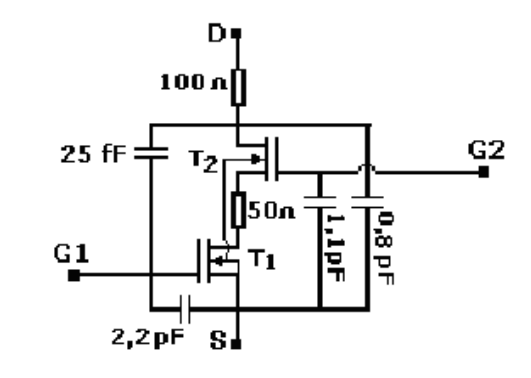
\includegraphics[scale=0.75]{circuitos/modelo_simplificado.png}
\caption{Modelo simplificado a utilizar}
\label{fig:modelo_simplificado}
\end{figure}

\subsubsection{Altas frecuencias sin considerar las puntas de prueba}

Reemplazando el modelo simplificado en el circuito se obtiene el modelo en señal
mostrado en la figura \ref{fig:circuito_alta_frec} para altas frecuencias.

\begin{figure}[H]
\centering
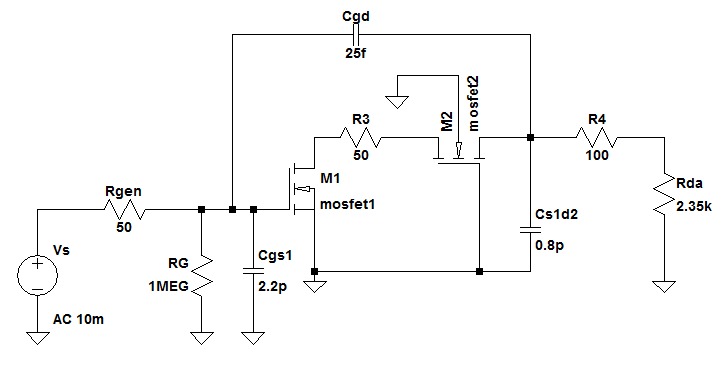
\includegraphics[scale=0.75]{circuitos/circuito_altas_frecuencias.png}
\caption{Circuito de señal para altas frecuencias}
\label{fig:circuito_alta_frec}
\end{figure}

Se obtendrán las constantes de tiempo asociadas a cada nodo del transistor.
Para obtener una frecuencia de corte superior $f_h$ mediante el método
de las constantes de tiempo.

\begin{itemize}
\item \textbf{Gate del transistor M1}

En este nodo se encuentra el capacitor $C_{gs1}$ y $C_{gd}$, para
el análisis se reflejará el capacitor $C_{gd}$ y se obtendrá su paralelo
con $C_{gs1}$.

\[ \displaystyle C_{gs1}^* = C_{gs1} + C_{gd} (1-A_{g1d2}) \]

Siendo $A_{g1d2}$ la amplificación total $A_v$ se obtiene:

\[ \displaystyle C_{gs1}^* = 2.2\,\unit{pF} + 0.025\,\unit{pF} (1+10.8) = 2.50\,\unit{pF} \]

La resistencia vista desde los terminales del capacitor $C_{gs1}$ es 
$R_{gs1} = 1\,\unit{M\Omega} // 50\,\unit{\Omega} \approx 50\,\unit{\Omega}$.
Se calcua la constante de tiempo:

\[ \displaystyle \tau_{gs1} = R_{gs1}\ C_{gs1} =  50\,\unit{\Omega}\ 2.50\,\unit{pF} =
125\,\unit{ps}\]

A esta constante de tiempo le corresponde la frecuencia:

\[ \displaystyle f_{gs1} = \frac{1}{2\ \pi \ \tau_{gs1}} =
\frac{1}{2\ \pi \ 125 \,\unit{ps}} = 1.27\,\unit{GHz} \]

\item \textbf{Source del transistor M1}

Los capacitores asociados a este nodo no son relevantes, ya que el nodo está
conectado a común. Por lo que su potencial esta definido y es constante.

\item \textbf{Gate del transistor M2}

Al igual que el caso anterior, este terminal está conectado a tierra. Por
lo que los capacitores asociados a este nodo no son relevantes.

\item \textbf{Drain del transistor M2}

En este nodo se encuentra $C_{gd}$ y $C_{s1d2}$, por lo que será necesario
reflejar $C_{gd}$ para que quede en paralelo con $C_{s1d2}$. Resultando:

\[ \displaystyle C_{ds2}^* = C_{s1d2} + C_{gd} (1 - A_{d2g1}) \]

Como $A_{d2g1}$ es la amplificación inversa del circuito. Resulta:

\[ \displaystyle A_{d2g1} = A_{d2d1} A_{d1g1} \]

Pero como $A_{d1g1}$ ya que desde el drain no se puede controlar al gate.
Por lo que resulta:

\[ \displaystyle A_{d2g1} = 0 \]

Finalmente:

\[ \displaystyle C_{ds2}^* = C_{s1d2} + C_{gd} = 0.8\,\unit{} + 0.025\,\unit{pF}
= 0.825\,\unit{pF}\]

La resistencia asociada se calcula mediante:

\[ \displaystyle R_{ds2} = 100\,\unit{\Omega} + 2.35\,\unit{k\Omega} = 2.45\,\unit{k\Omega} \]

Finalmente la constante de tiempo es:

\[ \displaystyle \tau_{ds2} = R_{ds2}\ C_{ds2} =  2.45\,\unit{k\Omega}\ 0.825\,\unit{pF} =
2.02\,\unit{ns}\]

Para esta constante de tiempo se obtiene la frecuencia:

\[ \displaystyle f_{ds2} = \frac{1}{2\ \pi \ \tau_{ds2}} =
\frac{1}{2\ \pi \ 2.02\,\unit{ns}} = 78.8\,\unit{MHz} \]

\end{itemize}

Como las frecuencias obtenidas están separadas por más de una década,
se tomará como frecuencia de corte la menor frecuencia. Por lo tanto:

\[ \displaystyle f_{h} = 78.8\,\unit{MHz} \]


\subsubsection{Altas frecuencias con puntas de prueba X10}

Se agregan al circuito los modelos equivalentes de las 
puntas X10 del osciloscopio, una a la entrada y otra a la salida. 
En la figura \ref{fig:altas_frec_puntaX10} se muestra el banco
de medición.


\begin{figure}[H]
\centering
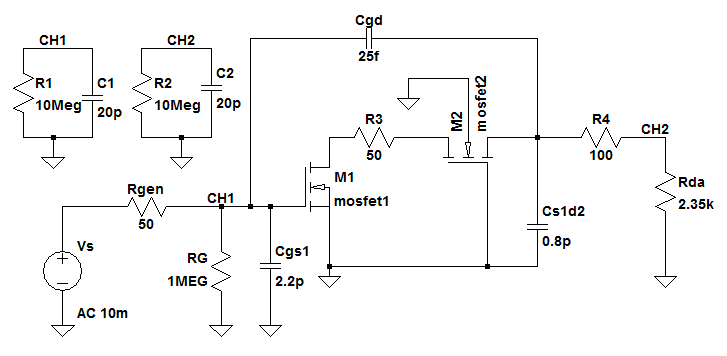
\includegraphics[scale=0.65]{circuitos/circuito_altas_frecuencias_puntaX10.png}
\caption{Circuito de señal para altas frecuencias considerando las puntas X10}
\label{fig:altas_frec_puntaX10}
\end{figure}

Teniendo en cuenta las puntas del osciloscopio, utilizando puntas x10. Se
agrega en la entrada y salida un capacitor $C_{punta} = 20\,\unit{pF}$
y una resistencia $R_{punta} = 10\,\unit{M\Omega}$, pero al agregarse
en paralelo a $R_s = 50\,\unit{\Omega}$ y $R_{da} = 2.45\,\unit{k\Omega}$
la resistencia de las puntas se considera despreciable. Por lo tanto solo
se sumará a los capacitores antes calculados el capacitor de las puntas.

Entonces:

\[ \displaystyle \tau_{gs1} = R_{gs1} (C_{gs1} + C_{punta}) = 
50\,\unit{\Omega}\ (2.50\,\unit{pF} + 20\,\unit{pF}) =
1.13\,\unit{ns}\]

A esta constante de tiempo le corresponde la frecuencia:

\[ \displaystyle f_{gs1} = \frac{1}{2\ \pi \ \tau_{gs1}} =
\frac{1}{2\ \pi \ 1.13 \,\unit{ns}} = 140\,\unit{MHz} \]

\[ \displaystyle \tau_{ds2} = R_{ds2} (C_{ds2} + C_{punta}) = 
2.45\,\unit{k\Omega}\ (0.825\,\unit{pF} + 20\,\unit{pF}) =
51.0\,\unit{ns}\]

A esta constante de tiempo le corresponde la frecuencia:

\[ \displaystyle f_{ds2} = \frac{1}{2\ \pi \ \tau_{ds2}} =
\frac{1}{2\ \pi \ 51.0 \,\unit{ns}} = 3.12\,\unit{MHz} \]

Como puede observarse de los valores calculados, las puntas
reducen considerablemente la frecuencia de corte superior $f_h$.
De haber calculado $f_h = 78.8\,\unit{MHz}$ teniendo en cuenta
las puntas del osciloscopio x10 se obtiene $f_h = 3.12\,\unit{MHz}$


\subsubsection{Altas frecuencias con punta de prueba activa}

Se reemplaza ahora el modelo equivalente de la punta de prueba X10 en la salida por una
el modelo equivalente de una punta de prueba activa. 
En la figura \ref{fig:altas_frec_punta_activa} se muestra el banco
de medición.


\begin{figure}[H]
\centering
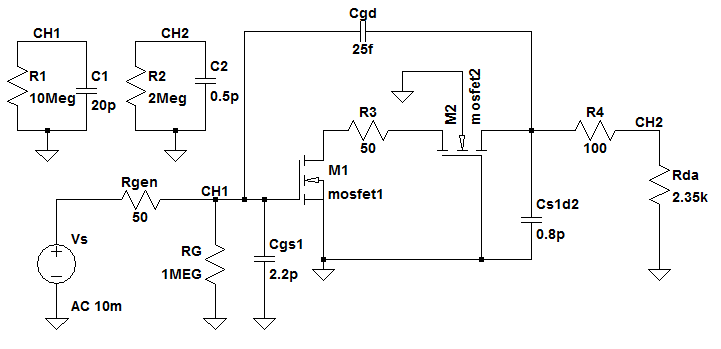
\includegraphics[scale=0.65]{circuitos/circuito_altas_frecuencias_punta_activa.png}
\caption{Circuito de señal para altas frecuencias con punta activa en la salida}
\label{fig:altas_frec_punta_activa}
\end{figure}

Para este caso solo se modifica el nodo de la salida. Ya que en la
entrada se sigue usando una punta de prueba X10. Por lo que se
repetirán las cuentas para el nodo de salida para la punta activa.

\[ \displaystyle \tau_{ds2} = R_{ds2} (C_{ds2} + C_{punta}) = 
2.45\,\unit{k\Omega}\ (0.825\,\unit{pF} + 0.5\,\unit{pF}) =
3.25\,\unit{ns}\]

En el nodo de la entrada se sigue obteniendo la misma constante
de tiempo ya que no se modifica la punta en este nodo.
Por lo que resulta:

\[ \displaystyle \tau_{gs1} = 1.13\,\unit{ns}\]

Como $\tau_{gs1}$ y $\tau_{ds2}$ son constantes de tiempo de valores
similares, se admite como valor aproximado una constante
de tiempo equivalente resultado de la suma de los valores individuales.

Resultando:

\[ \displaystyle \tau_h = \tau_{gs1} + \tau_{ds2} = 1.13\,\unit{ns} + 3.25\,\unit{ns} = 4.48\,\unit{ns} \]

Que corresponde a la frecuencia:

\[ \displaystyle f_h = \frac{1}{2\ \pi\ \tau_h} = \frac{1}{2\ \pi\ 4.48\,\unit{ns}} \]

Resultando la frecuencia de corte superior:

\[ \displaystyle f_h = 35.5\,\unit{MHz} \]

De este resultado se observa que utilizando puntas activas se
obtiene un resultado mas cercano al ideal sin usar puntas. Ya
que el valor obtenido es mas cercano al calculado sin considerar
las puntas($78.8\,\unit{MHz}$) que el obtenido utilizando puntas
X10($3.12\,\unit{MHz}$).

\subsubsection{Bajas frecuencias}
Utilizando el circuito de la figura \ref{fig:circuitototal} se calculan las constantes de tiempo asociadas a cada capacitor.


\begin{itemize}

\item \textbf{Capacitor CG}
Para calcular la constante de tiempo asociada a este capacitor Se coloca una fuente de tensión de prueba desde el terminal marcado como J1. Desde este terminal, y considerando las resistencias gate-drain y gate-source del transistor 2 como infinitas, se observa la siguiente resistencia:

\[ \displaystyle R_{CG} = \frac{r_{gs}+R_{G}}{\beta_{FET}}//R_{S}= \frac{1}{g_{m1}}//R_{S} = 178\,\unit{\Omega} \]

La resistencia vista desde este terminal no variara si se conectan tanto la punta x1 como la punta x10 a la entrada debido a que el capacitor que introduce se encuentra en paralelo con el camino de la señal (es de altas frecuencias), y la resistencia que se introduce es despreciable al dividir todo por $\beta_{FET}$. Por lo tanto la constante de tiempo obtenida es:

\[ \displaystyle \tau_{CG} = R_{CG} C_{CG} = 
178\,\unit{\Omega}\ 1\,\unit{uF} =
178\,\unit{us}\]

por lo tanto la frecuencia que se obtiene es:
\[ \displaystyle f_{CG} = \frac{1}{2\ \pi \ \tau_{CG}} =
\frac{1}{2\ \pi \ 178 \,\unit{us}} = 894\,\unit{Hz} \]

\item \textbf{Capacitor CL}
Este capacitor posee conectado en serie la resistencia de salida del circuito (que se calculo anteriormente) y la resistencia de carga $R_L$, por lo tanto la resistencia resultante es:

\[ \displaystyle R_{CL} =R_{o}+R_{L} =4.7\,\unit{k\Omega} + 4.7\,\unit{k\Omega} = 9.4\,\unit{k\Omega} \]

Por lo que la constante de tiempo resultante es:
\[ \displaystyle \tau_{CL} = R_{CL} C_{L} = 
9.4\,\unit{k\Omega}\ 1\,\unit{uF} =
9.4\,\unit{ms}\]

En este caso, al conectar la punta x1 o x10 a la salida, el valor no se modifica. Esto se debe a que queda una resistencia de $1\,\unit{M\Omega}$ en paralelo a la resistencia de carga en el caso de utilizar punta x1, y una de $10\,\unit{M\Omega}$ en el caso de utilizar punta x10, valores mucho mayores que $4.7\,\unit{k\Omega}$. En el caso del capacitor en paralelo que se agrega, su valor será de $200\,\unit{pF}$ en la punta x1, y de $20\,\unit{pF}$ en la punta x10, por lo que se observa que al sumar este valor al capacitor $C_L$, su valor prácticamente o se modifica. Por lo tanto la frecuencia obtenida es:

\[ \displaystyle f_{CL} = \frac{1}{2\ \pi \ \tau_{CL}} =
\frac{1}{2\ \pi \ 9.4 \,\unit{ms}} = 17\,\unit{Hz} \]

\end{itemize}

Debido a que la frecuencia asociada al capacitor $C_G$ es mucho mayor que la asociada al capacitor $C_L$, se toma como frecuencia de corte inferior $f_L= 894\,\unit{Hz}$. Por otro lado puede verse que las puntas de osciloscopio no influyen al analizar bajas frecuencias.



\section{Simulación}

\subsection{Punto de reposo}
Para simular el punto de reposo (comando \texttt{.op} del LTSpice) se utiliza el circuito
de la figura \ref{fig:SIMUreposo}. Cabe aclarar que mediante el comando \texttt{.model} se
modificaron los parámetros de ambos transistores de acuerdo a los que se utilizaron en
el calculo analítico. En la tabla \ref{table:valoresreposoSIMU} se observan las
tensiones y corrientes obtenidas. Puede verse que no hay gran diferencia con lo
calculado en la sección anterior.


\begin{figure}[H]
\centering
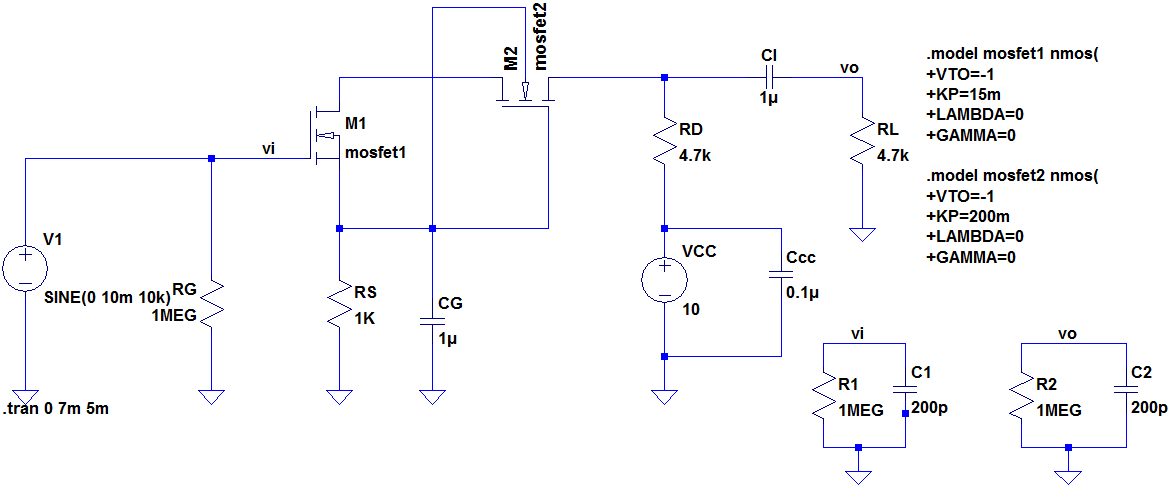
\includegraphics[scale=0.5]{circuitos/circuitosimuOP.png}
\caption{Circuito para simular el punto de reposo}
\label{fig:SIMUreposo}
\end{figure}

\begin{table}[H]
\centering
\begin{tabular}{|c|c|c|c|c|c|c|} 
\hline
Transistor & $V_{G}$ & $V_{S}$ & $V_{D}$ & $I_{D}$ & $V_{GS}$ & $V_{DS}$  \\ \hline
M1 & $0\,\unit{V}$ & $0.70\,\unit{V}$  & $1.61\,\unit{V}$ & $0.7\,\unit{mA}$ & $-0.7\,\unit{V}$  & $0.91\,\unit{V}$ \\ \hline
M2 & $0.7\,\unit{V}$ & $1.61\,\unit{V}$ & $6.73\,\unit{V}$ & $0.7\,\unit{mA}$ & $-0.91\,\unit{V}$ & $5.12\,\unit{V}$\\ \hline
\end{tabular}
\caption{Corrientes y tensiones contra común en reposo simuladas}
\label{table:valoresreposoSIMU}
\end{table}

\subsection{Amplificación de tensión total (\texorpdfstring{$A_v$}{TEXT}) a frecuencias medias}

Para calcular la ganancia del circuito \ref{fig:SIMUreposo}  mediante simulación, se
simularon $2\,\unit{ms}$ de la señal, a partir de los $3\,\unit{ms}$ (para evitar el
transitorio) a $5\,\unit{KHz}$ (frecuencia que se tomo como frecuencia media) con
$10\,\unit{mV}$ de tensión. Se considero que utiliza punta x1 para medir tanto la
tensión se salida como la de entrada. La señal que se obtuvo puede observarse en la
figura \ref{fig:SIMUAvmedias}. De la misma se obtiene que la ganancia es
aproximadamente de -10 (ver que las señales están en contrafase).


\begin{figure}[H]
\centering
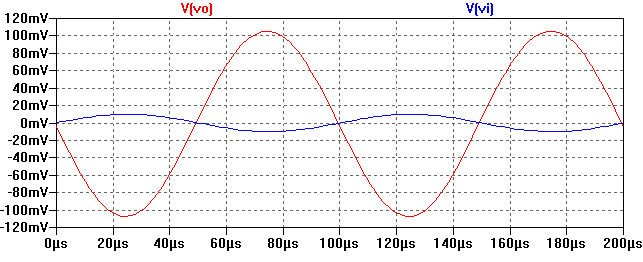
\includegraphics[scale=0.8]{senales/Avmedias.png}
\caption{Señales de entrada y salida para frecuencias medias}
\label{fig:SIMUAvmedias}
\end{figure}

\subsection{Resistencia de entrada y de salida}

Para la simulación de resistencia de entrada se armó el siguiente esquemático en LTspice:

\begin{figure}[H]
\centering
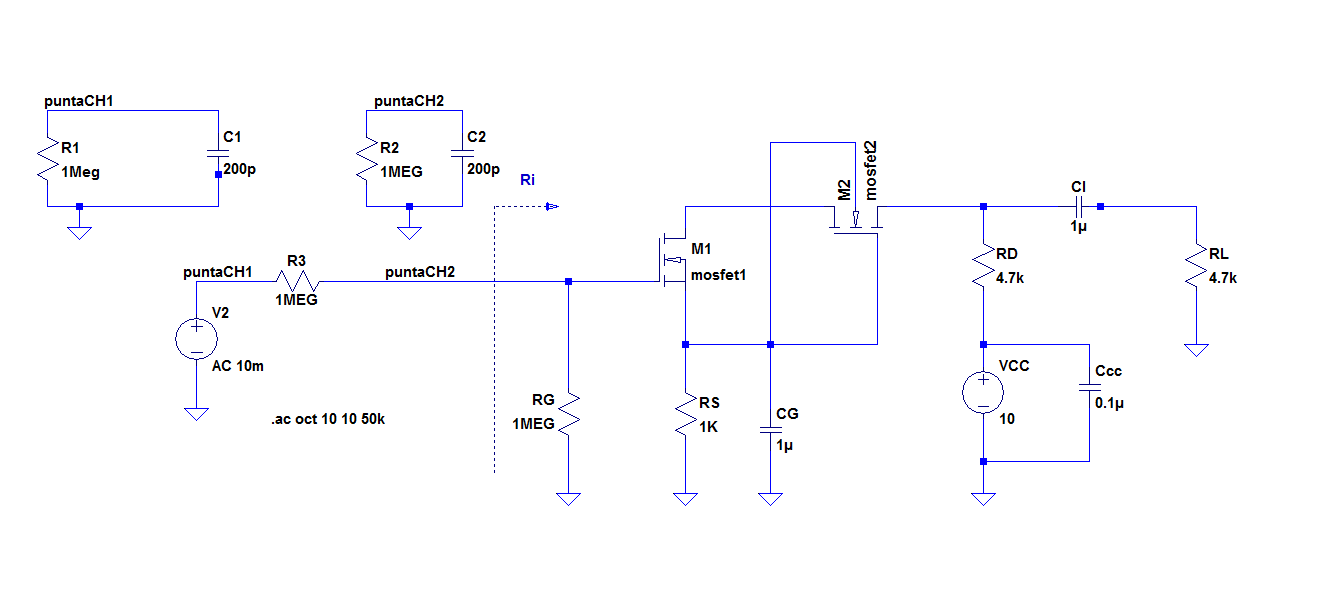
\includegraphics[scale=0.45]{circuitos/Esquematico-sim-Ri-con-punta.png}
\caption{Banco de medición para resistencia de entrada $R_{i}$.}
\label{fig:Ritotal}
\end{figure}

Haciendo un análisis AC se grafica $\frac{V_i}{I_i}$ en un rango apropiado de frecuencias.
Teniendo en cuenta que las mediciones estarán afectadas por los instrumentos, se incluyó en el modelado un equivalente de una punta de osciloscopio para verificar cómo se afectan. A continuación los resultados obtenidos en cada caso:

\begin{figure}[H]
\centering
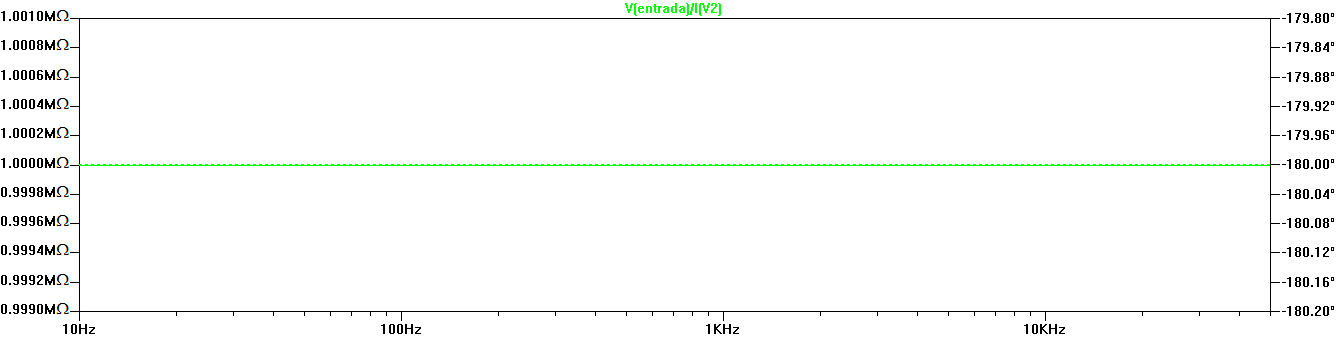
\includegraphics[scale=0.45]{senales/simulacion-Ri-sin-punta.png}
\caption{Resistencia de entrada simulada desconectando el equivalente de la punta de osciloscopio.}
\label{fig:SIMURi_sin_punta}
\end{figure}

El resultado obtenido en este caso coincide con el predicho por el análisis por inspección.

\begin{figure}[H]
\centering
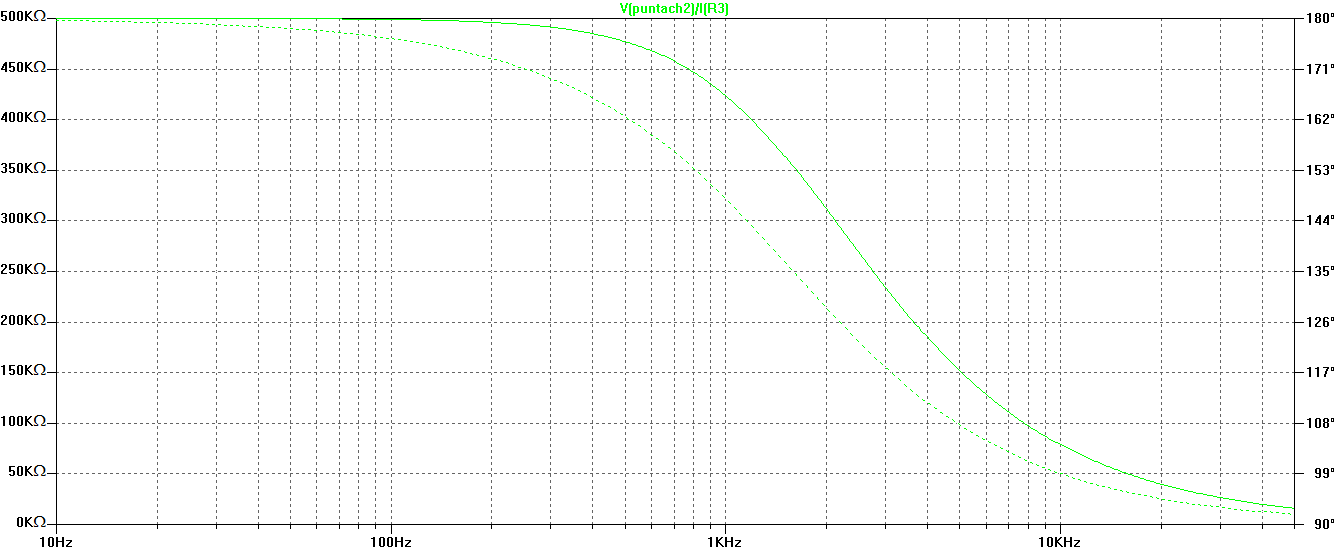
\includegraphics[scale=0.45]{senales/simulacion-Ri-con-punta.png}
\caption{Resistencia de entrada simulada teniendo en cuenta el equivalente de la puntaX1 de osciloscopio.}
\label{fig:SIMURi_con_puntax1}
\end{figure}

En este caso se puede notar cómo a frecuencias bajas la resistencia equivalente de la punta afectaría la medición resultando el paralelo del valor real con el de dicha resistencia.Es decir:

\[ \displaystyle R_{medida}=R_{punta}//R_{i}=1\,\unit{M\Omega}//1\,\unit{M\Omega}=500\,\unit{k\Omega} \]

Además también se puede notar cómo la capacidad asociada a la punta hace que a partir de frecuencias un poco menores que la de corte del filtro formado  ($F_{corte}=1,5\unit{kHz}$) la medición se desvíe del valor real.
De manera análoga pero con una aproximación mucho mejor, la medición con una puntaX10 también afectaría el valor obtenido, como se muestra en la siguiente simulación.

\begin{figure}[H]
\centering
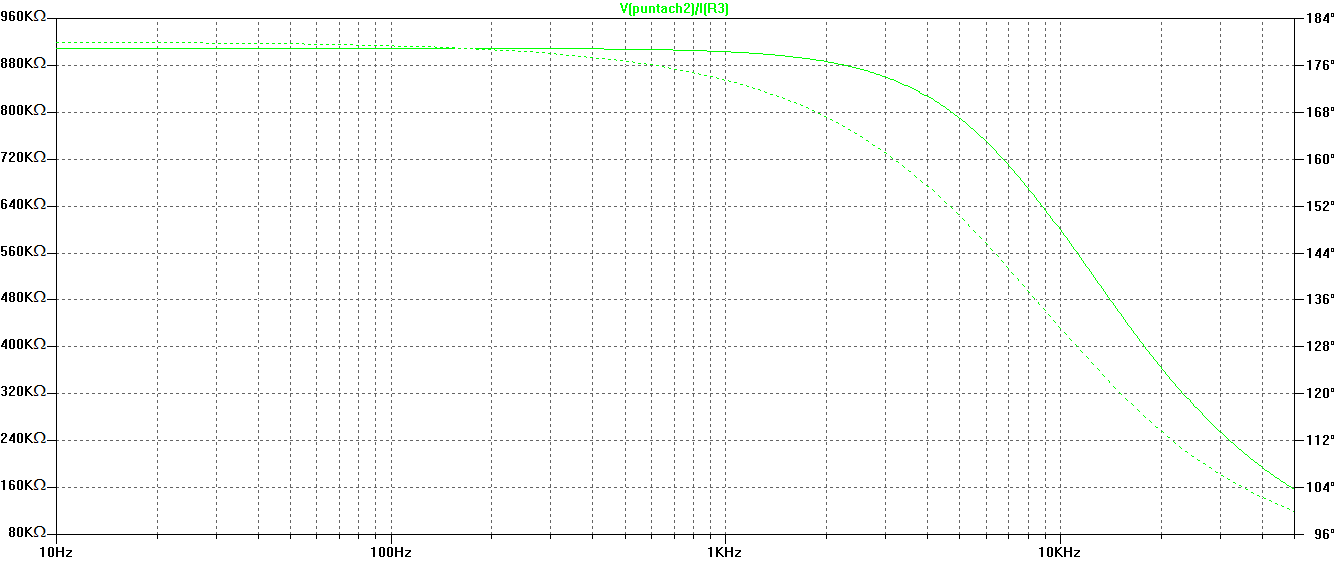
\includegraphics[scale=0.45]{senales/simulacion-Ri-con-puntax10.png}
\caption{Resistencia de entrada simulada teniendo en cuenta el equivalente de la puntaX10 de osciloscopio.}
\label{fig:SIMURi_con_puntax10}
\end{figure}

Para éste caso la resistencia estimada no estaría tan lejos del valor real($910k\Omega$) ya que la punta x10 tiene una resistencia equivalente mayor.

Para la resistencia de salida el banco de medición modelado es el siguiente:


\begin{figure}[H]
\centering
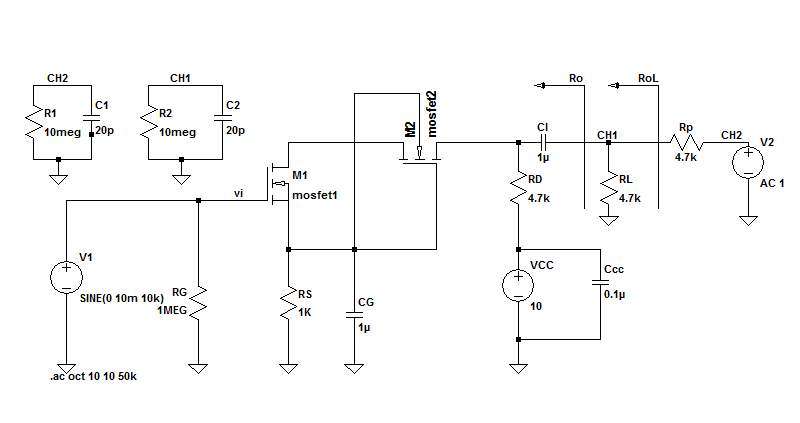
\includegraphics[scale=0.75]{circuitos/Esquematico-simulacion-Ro.png}
\caption{Banco de medición para resistencia de salida $R_{o}$.}
\label{fig:Rototal}
\end{figure}

Como la resistencia $R_L$ está soldada a la placa que se utilizará
para la medición, esta no podría removerse para la medición de $R_o$.
Por lo que se obtendrá primero la resistencia $R_{oL}$ y luego
se despejará $R_o$ del paralelo $R_{oL} = R_L // R_o$.

Procediendo de manera análoga que para el caso de la resistencia de entrada los resultados obtenidos fueron los siguientes:


\begin{figure}[H]
\centering
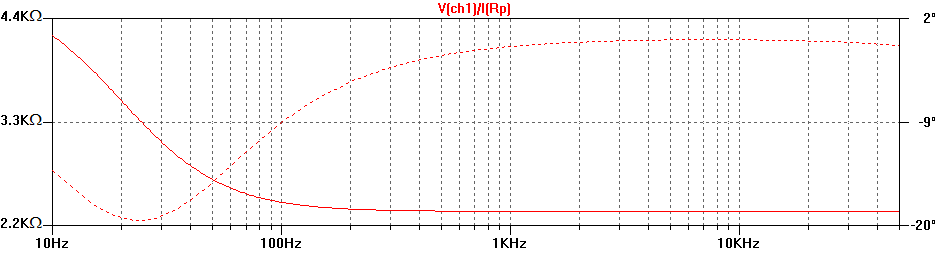
\includegraphics[scale=0.6]{senales/simulacion-Ro.png}
\caption{Resistencia de salida en paralelo a $R_L$ simulada teniendo en cuenta el equivalente de la punta de osciloscopio.}
\label{fig:SIMURo_con_punta}
\end{figure}

El resultado hallado es de $R_{oL}=2,35\unit{k\Omega}$.
Por lo que si $R_L = 4,7\unit{k\Omega}$ la resistencia
de salida es $R_o = 4,7\unit{k\Omega}$.


\subsection{Excursión de salida}

\subsubsection{Máxima excursión de salida sin distorsión}

A partir del mismo esquemático presentado en la sección anterior, se verificó el
límite de distorsión aceptable calculado anteriormente variando la amplitud de la
señal de entrada.


\begin{figure}[H]
\centering
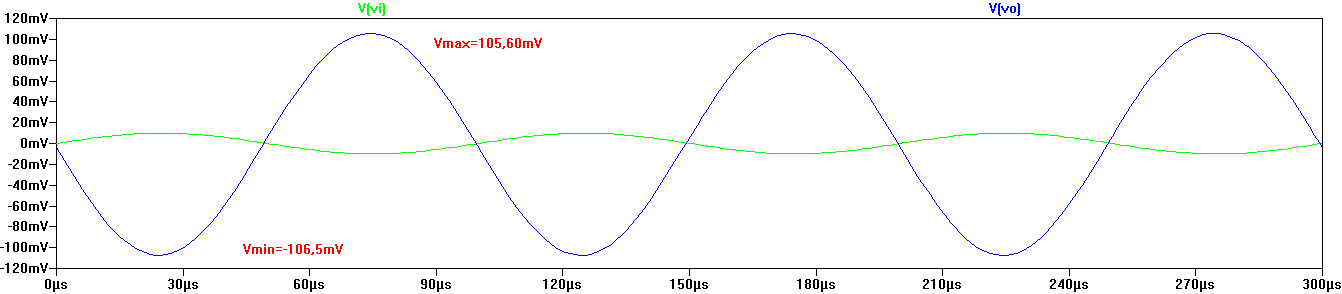
\includegraphics[scale=0.45]{senales/simulacion-max-exc-sin-distorsion.png}
\caption{$V_{in}$ y $V_{out}$  para una señal de entrada de frecuencia 5\unit{kHz} y 10\unit{mV} de amplitud.}
\label{fig:SIMUmax_sin_distorsion}
\end{figure}


En la figura \ref{fig:SIMUmax_sin_distorsion} la distorsión no es apreciable a simple vista, sin embargo al aumentar  la amplitud empieza a notarse cada vez más, como se ve en la figura \ref{fig:SIMUmax_con_distorsion}.

\begin{figure}[H]
\centering
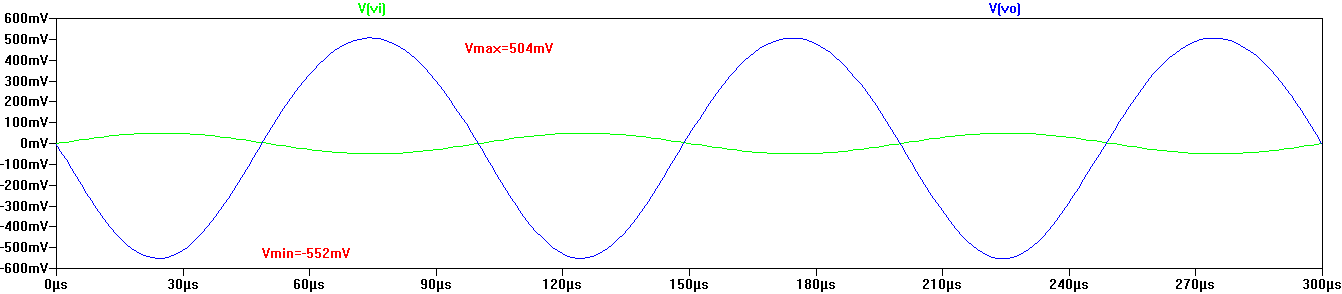
\includegraphics[scale=0.45]{senales/simulacion-max-exc-con-distorsion.png}
\caption{$V_{in}$ y $V_{out}$  para una señal de entrada de frecuencia  5\unit{kHz}  y  amplitud  50\unit{mV} .}
\label{fig:SIMUmax_con_distorsion}
\end{figure}

Mediante el comando \texttt{.FOUR} de Spice se obtienen
los componentes de Fourier de la señal de salida, para
analizar la distorsión. 

En la tabla \ref{table:tabla_four} se muestran los resultados obtenidos para una 
señal de entrada de amplitud $15,\unit{mV}$ y frecuencia $5\,\unit{kHz}$. 
Se obtiene una distorsión armónica total de $1.20\,\unit{\%}$.

\begin{table}[H]
\centering
\begin{tabular}{|c|c|c|c|c|c|} 
\hline
Harmonic & Frequency & Fourier & Normalized	& Phase	& Normalized \\
  & [kHz] & Component & Component	&  	& Phase \\ \hline

1	&	$	5.00	$	&	$	1.58E-01	$	&	$	1.00E+00	$	&	$	    7.55	^\circ	$	&	$	    0.00	^\circ	$	\\ \hline
2	&	$	10.0	$	&	$	1.90E-03	$	&	$	1.20E-02	$	&	$	  109.01	^\circ	$	&	$	  101.46	^\circ	$	\\ \hline
3	&	$	15.0	$	&	$	4.44E-06	$	&	$	2.81E-05	$	&	$	  -44.50	^\circ	$	&	$	  -52.05	^\circ	$	\\ \hline
4	&	$	20.0	$	&	$	1.27E-06	$	&	$	8.02E-06	$	&	$	  173.58	^\circ	$	&	$	  166.02	^\circ	$	\\ \hline
5	&	$	25.0	$	&	$	1.21E-06	$	&	$	7.69E-06	$	&	$	   -5.50	^\circ	$	&	$	  -13.05	^\circ	$	\\ \hline
6	&	$	30.0	$	&	$	1.06E-06	$	&	$	6.74E-06	$	&	$	 -178.68	^\circ	$	&	$	 -186.23	^\circ	$	\\ \hline
7	&	$	35.0	$	&	$	1.09E-06	$	&	$	6.92E-06	$	&	$	    5.15	^\circ	$	&	$	   -2.40	^\circ	$	\\ \hline
8	&	$	40.0	$	&	$	9.71E-07	$	&	$	6.15E-06	$	&	$	 -166.78	^\circ	$	&	$	 -174.34	^\circ	$	\\ \hline
9	&	$	45.0	$	&	$	1.02E-06	$	&	$	6.48E-06	$	&	$	   19.02	^\circ	$	&	$	   11.47	^\circ	$	\\ \hline
10	&	$	50.0	$	&	$	9.12E-07	$	&	$	5.78E-06	$	&	$	 -152.35	^\circ	$	&	$	 -159.91	^\circ	$	\\ \hline
\multicolumn{6}{|c|}{Total Harmonic Distortion: $1.200853\%(1.202284\%)$}\\ \hline
\end{tabular}
\caption{Resultados obtenidos mediante el comando \texttt{.FOUR}}
\label{table:tabla_four}
\end{table}

En la figura \ref{fig:fft} se grafican las componentes de Fourier obtenidas 
del comando \texttt{.FOUR}. 
Y en la figura \ref{fig:fft_ruido} se omite la frecuencia del generador para
mostrar las componentes que originan la distorsión en la señal de salida.

\begin{figure}[H]
\centering
\begin{subfigure}{.5\textwidth}
  \centering
  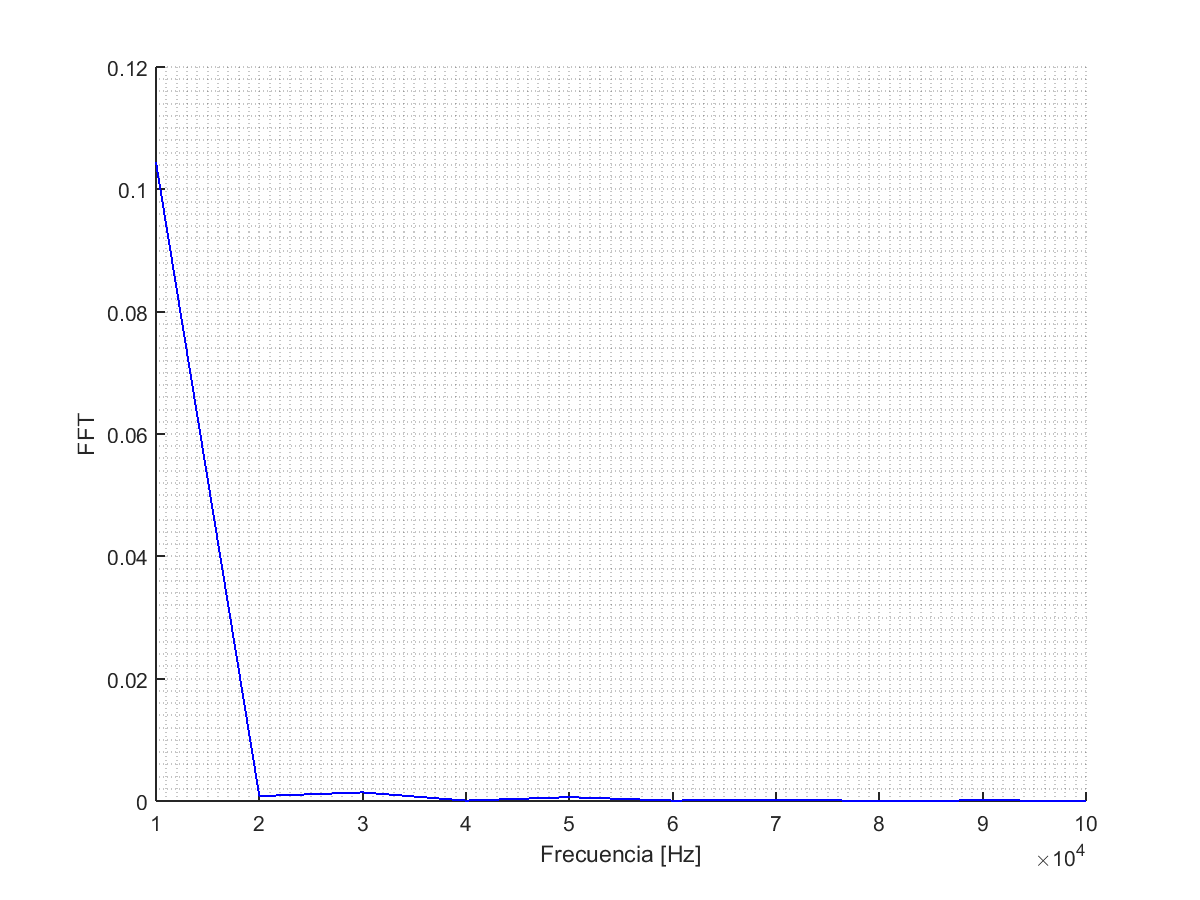
\includegraphics[width=1\linewidth]{curvas/fft.png}
  \caption{De la señal de salida.}
  \label{fig:fft}
\end{subfigure}%
\begin{subfigure}{.5\textwidth}
  \centering
  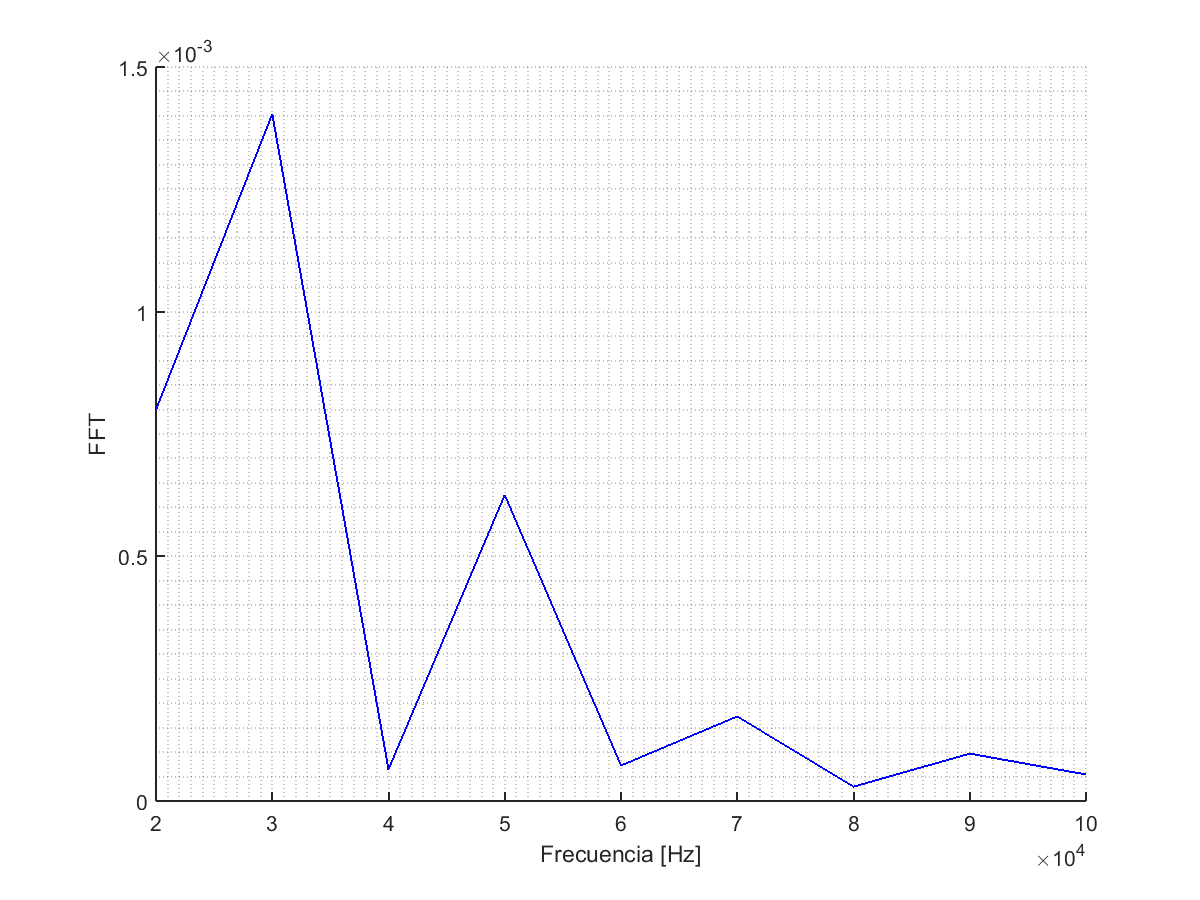
\includegraphics[width=1\linewidth]{curvas/fft_ruido.png}
  \caption{De la señal de salida omitiendo la frecuencia del generador.}
  \label{fig:fft_ruido}
\end{subfigure}
\caption{Componentes de Fourier.}
\end{figure}


\subsubsection{Máxima excursión de salida sin recorte}

Finalmente para comprobar $V_{o_{max}}$ al recortar la señal de salida se repitió la simulación \texttt{.trans} hasta lograr ver dicho efecto. La amplitud de entrada necesaria para divisarlo fue $\widehat{V_s}=220\,\unit{mV}$, valor distinto al calculado teóricamente ya que como la señal se encuentra muy distorsionada para esta amplitud de entrada, el valor de $A_v$ calculado puede variar.

\begin{figure}[H]
\centering
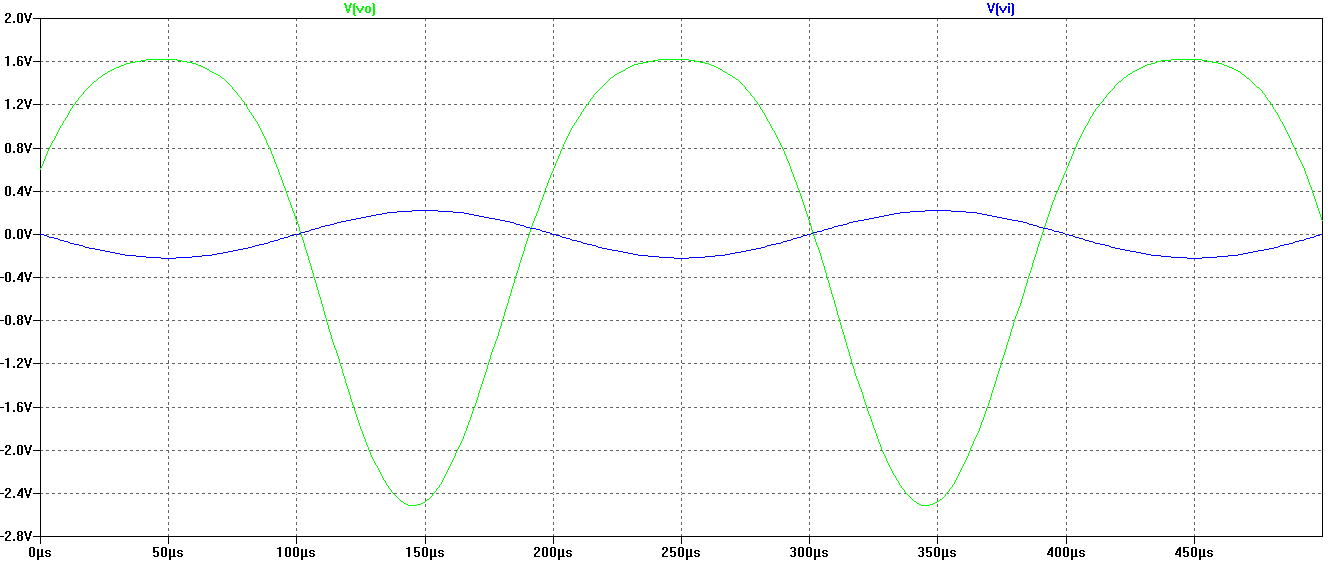
\includegraphics[scale=0.45]{senales/simulacion-vomax-recorte.png}
\caption{$V_{in}$ y $V_{out}$  para una señal de entrada de frecuencia  5\unit{kHz}  y  amplitud  220\unit{mV} .}
\label{fig:SIMUmax_corte}
\end{figure}





\subsection{Respuesta en frecuencia de  \texorpdfstring{$A_{vs}$}{TEXT}}

Se simula mediante la instrucción \textbf{.ac} de LTSpice, cambiando los equivalentes conectados representando los diferentes tipos de punta que se utilizarán en las mediciones. En este caso se incluyeron en el modelado los capacitores que afectan la respuesta en alta frecuencia, indicados en el enunciado, para modelar las capacidades internas del \textbf{BF966}.

\begin{figure}[H]
\centering
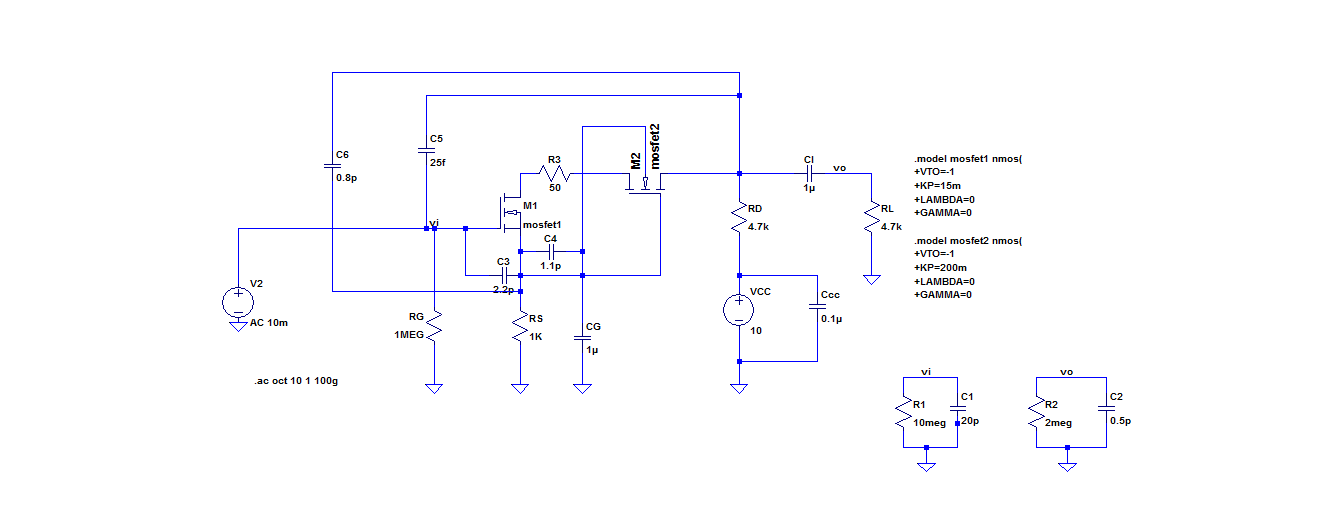
\includegraphics[scale=0.45]{circuitos/Esquematico-sim-Avs-rta-frec.png}
\caption{Esquematico de simulación de respuesta en frecuencia de Avs, equivalentes punta x10 y punta activa.}
\label{fig:EsquemAvs_rta_frec}
\end{figure}

Primero se muestra la respuesta en frecuencia real simulada, o sea sin conectar ningun equivalente que cargue al circuito.

\begin{figure}[H]
\centering
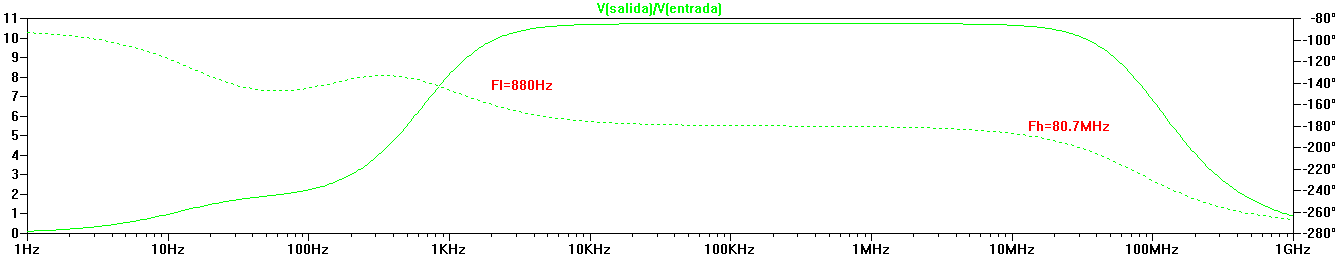
\includegraphics[scale=0.45]{senales/Avs_rta_frec_sin_punta.png}
\caption{Respuesta en frecuencia de $A_{vs}$ sin cargar el circuito}
\label{fig:SIMUAvs_rta_frec}
\end{figure}

A continuación cargando el circuito con los equivalentes de distintos tipos de punta. 



\begin{figure}[H]
\centering
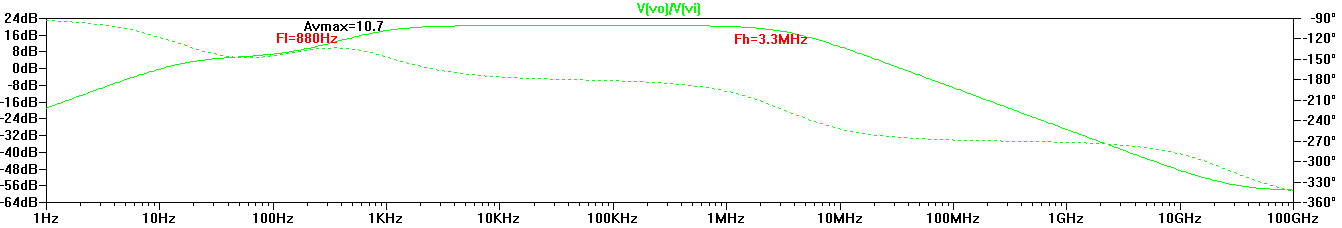
\includegraphics[scale=0.45]{senales/Avs_rta_frec_con_puntax10.png}
\caption{Respuesta en frecuencia de $A_{vs}$ conectando equivalentes punta x10.}
\label{fig:SIMUAvs_rta_frec_con_puntax10}
\end{figure}

\begin{figure}[H]
\centering
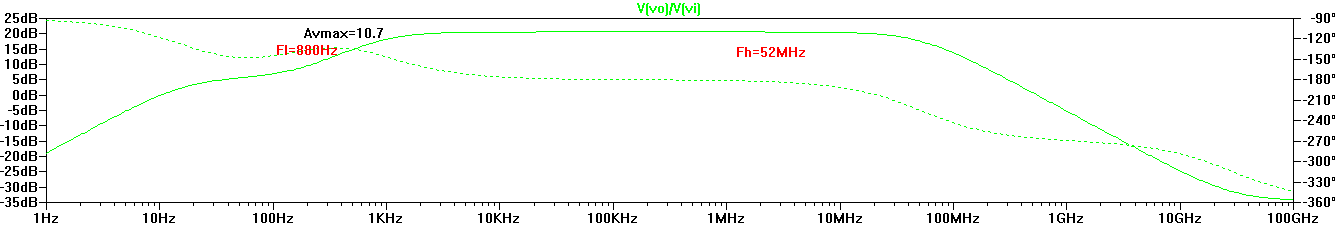
\includegraphics[scale=0.45]{senales/Avs_rta_frec_con_punta_activa.png}
\caption{Respuesta en frecuencia de $A_{vs}$ conectando equivalente puntax10 a la entrada y equivalente punta activa a la salida.}
\label{fig:SIMUAvs_rta_frec_con_punta_activa}
\end{figure}

A partir de los resultados de las simulaciones en un rango de frecuencias amplio se decide usar como frecuencia de medición para $R_i$ y $R_o$ 5 \unit{kHz}, ya que para este valor todas las magnitudes permanecen estables.


\section{Mediciones}

Para realizar las mediciones se utilizo el circuito impreso mostrado en la figura \ref{fig:impreso}

\begin{figure}[H]
\centering
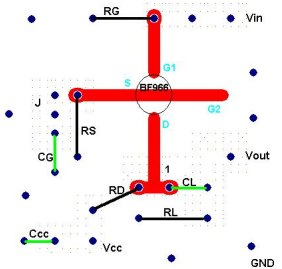
\includegraphics[scale=0.8]{circuitos/Impreso.png}
\caption{Circuito impreso utilzado}
\label{fig:impreso}
\end{figure}

\subsection{Punto de reposo}

De la medición del circuito de la figura \ref{fig:impreso} se obtienen los valores de la tabla \ref{table:valoresreposomedidos}. Tanto la tensión de drain del primer transistor como la tensión de source del segundo no se pueden medir. Esto se debe a que el circuito con el que se hizo el calculo analítico y posterior simulación representa un modelo del transistor integrado, por lo que los terminales nombrados anteriormente son inaccesibles.

\begin{table}[H]
\centering
\begin{tabular}{|c|c|c|c|c|c|c|} 
\hline
Transistor & $V_{G}$ & $V_{S}$ & $V_{D}$ & $I_{D}$ & $V_{GS}$ & $V_{DS}$  \\ \hline
M1 & $0\,\unit{V}$ & $0.55\,\unit{V}$  & - & $0.57\,\unit{mA}$ & $-0.55\,\unit{V}$  & - \\ \hline
M2 & $0.55\,\unit{V}$ & - & $7.4\,\unit{V}$ & $0.57\,\unit{mA}$ & - & -\\ \hline
\end{tabular}
\caption{Corrientes y tensiones contra común en reposo}
\label{table:valoresreposomedidos}
\end{table}

\subsection{Amplificación de tensión total (\texorpdfstring{$A_v$}{TEXT}) a frecuencias medias}

De la medición (ver figura \ref{fig:medicion_Avmedias}) del circuito de la figura \ref{fig:impreso} a $5\,\unit{KHz}$ con una tensión de entrada de aproximadamente $17\,\unit{mV}$, utilizando puntas de prueba X1, se obtuvo una ganancia de:

\[ \displaystyle A_{V} = \frac{v_o}{v_i} = -6.78 \]

\begin{figure}[H]
\centering
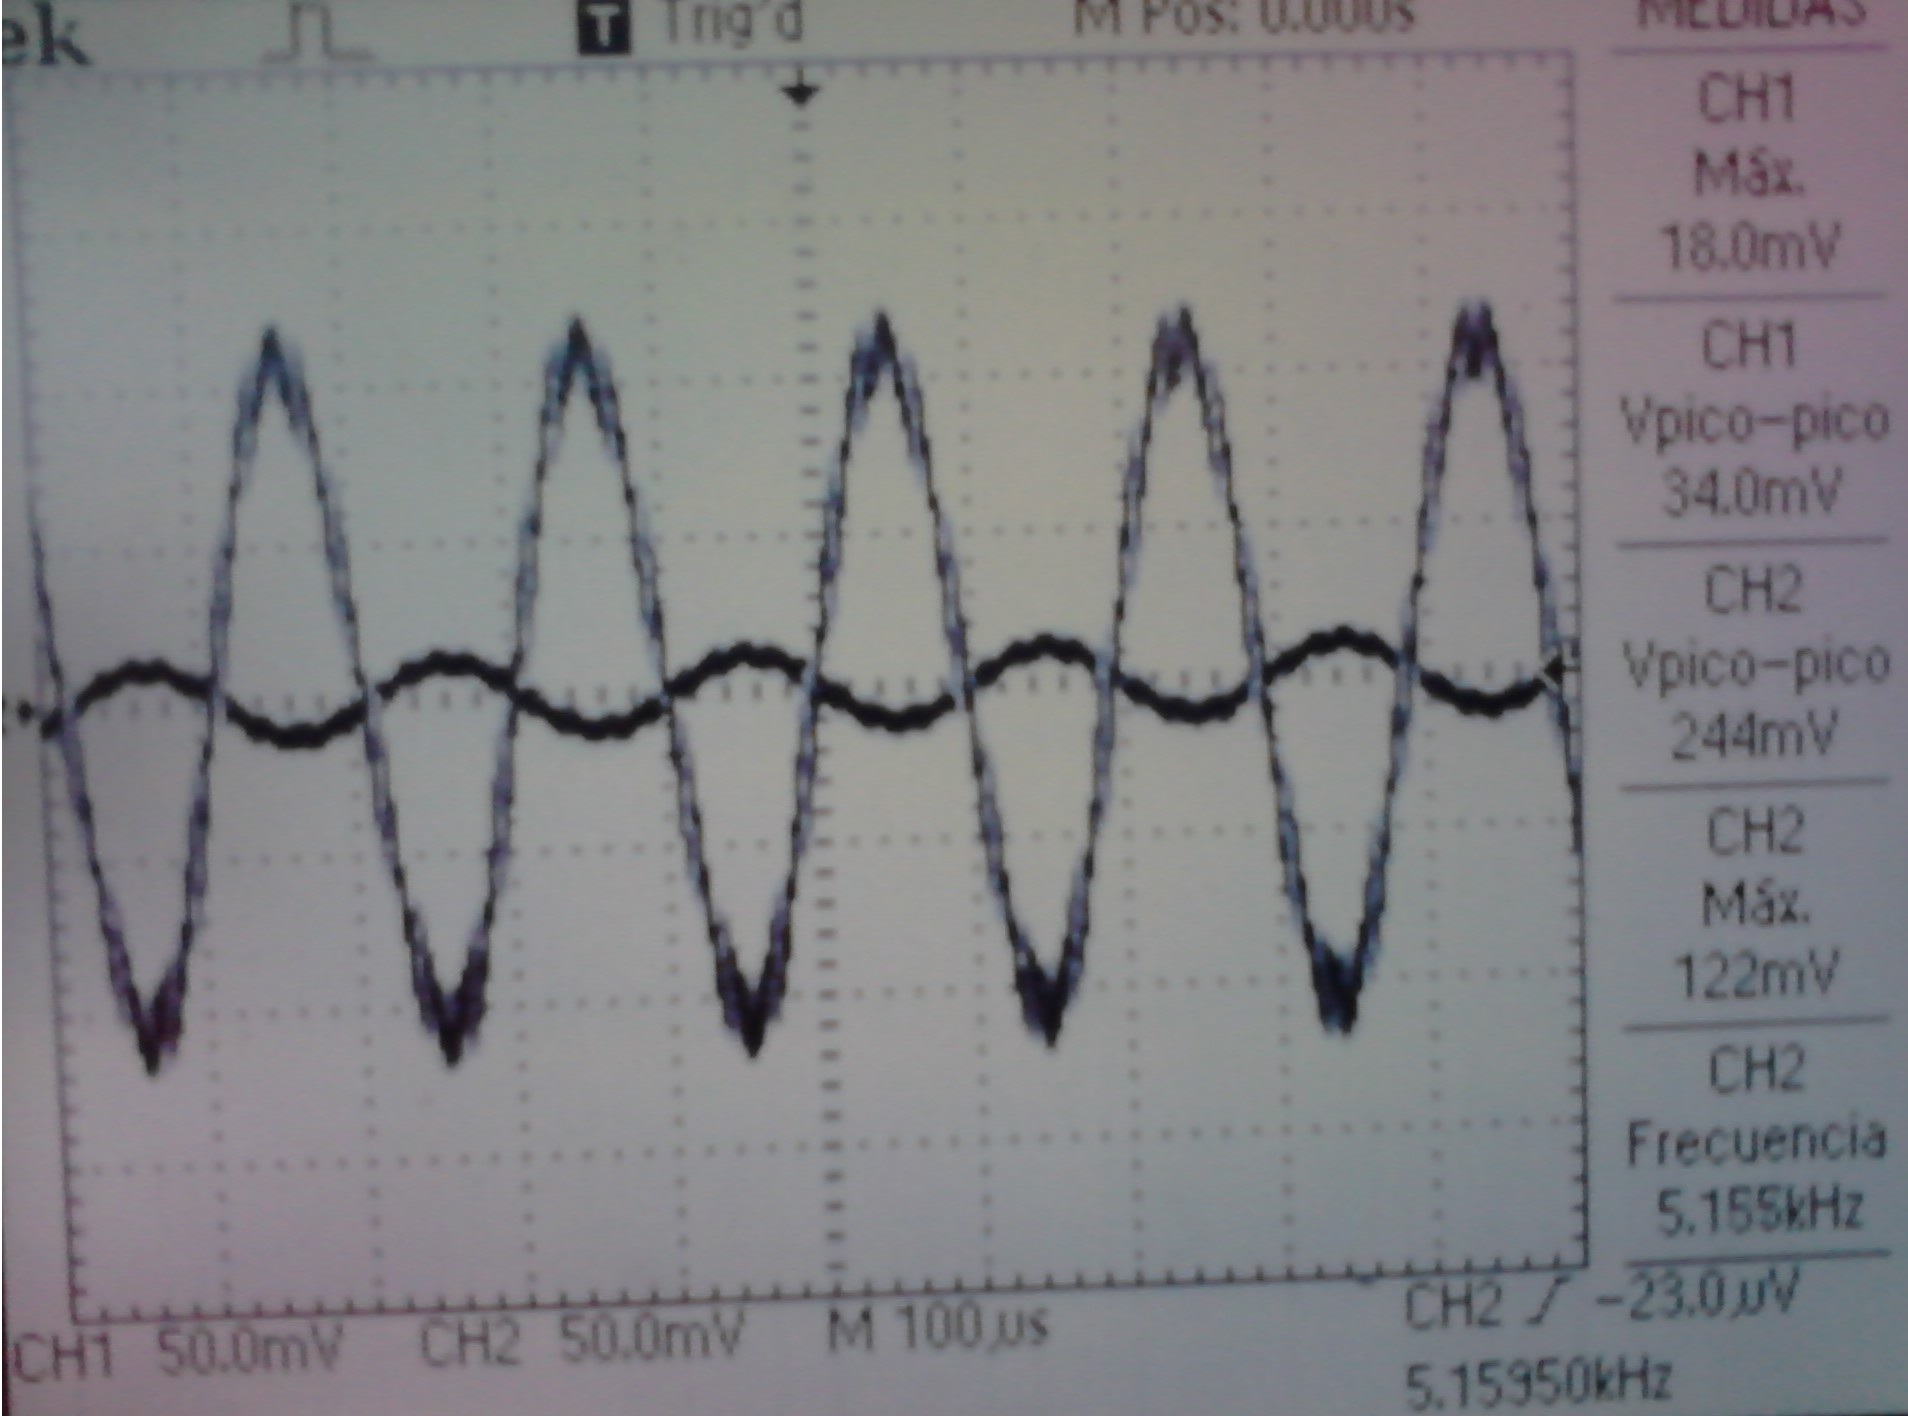
\includegraphics[scale=0.12]{mediciones/Av_medias_puntaX1_5kHz.jpg}
\caption{}
\label{fig:medicion_Avmedias}
\end{figure}


\subsection{Resistencia de entrada y salida}

\subsubsection{Resistencia de entrada \texorpdfstring{$R_i$}{TEXT}}

Utilizando el banco de medición de la figura \ref{fig:Ritotal} se
obtuvo la resistencia de entrada del circuito utilizando puntas
de prueba X1 y X10.

Se calcula la resistencia de entrada $R_i$ mediante la ecuación \ref{eq:Ri_medicion} utilizando valores picos para las tensiones.

\begin{equation}
    R_i = \frac{R_{prueba} V_{CH2}}{V_{CH1} - V_{CH2}}
   \label{eq:Ri_medicion}
\end{equation}


En la figura \ref{fig:medicion_Ri_X1} se muestran las curvas obtenidas
en el osciloscopio utilizando puntas de prueba X1 utilizando
una señal de entrada senoidal de $160\,\unit{mV}$ pico a una
frecuencia de $5\,\unit{kHz}$.

Con los valores picos de las mediciones se cacula:

\[ \displaystyle     R_i = \frac{1\,\unit{M\Omega}\  38.0\,\unit{mV}}{160\,\unit{mV} - 38.0\,\unit{mV}} 
\approx 311\,\unit{k\Omega}\]

El valor obtenido de $R_i$ con puntas X1 es mucho menor al calculado,
sin tener en cuenta la influencia de las puntas de prueba.
Las puntas de prueba X1 se modelan mediante
una resistencia de $1\,\unit{M\Omega}$ 
en paralelo a un capacitor de $200\,\unit{pF}$.

A la frecuencia de trabajo de $5\,\unit{kHz}$ el capacitor tiene
una reactancia de $1\,\unit{M\Omega}$. Por lo que al estar en paralelo
a la resistencia de $1\,\unit{M\Omega}$ de la punta se obtiene
una resistencia equivalente de $500\,\unit{k\Omega}$. Esto afecta considerablemente
a las mediciones realizadas, ya que se esta midiendo la tensión
entre los bornes de una resistencia de $1\,\unit{M\Omega}$ con
un instrumento que tiene una reactancia de entrada de
$500\,\unit{k\Omega}$.
Por lo que la punta del CH2 al agregarse en paralelo a $R_i$
modifica su valor, resultando:

\[ \displaystyle R_{i\ modificado} = R_{i\ teorico} // 500\,\unit{k\Omega}
= 1\,\unit{M\Omega} // 500\,\unit{k\Omega} \approx 333\,\unit{k\Omega} \]

Que es un valor similar al obtenido en la medición.

\begin{figure}[H]
\centering
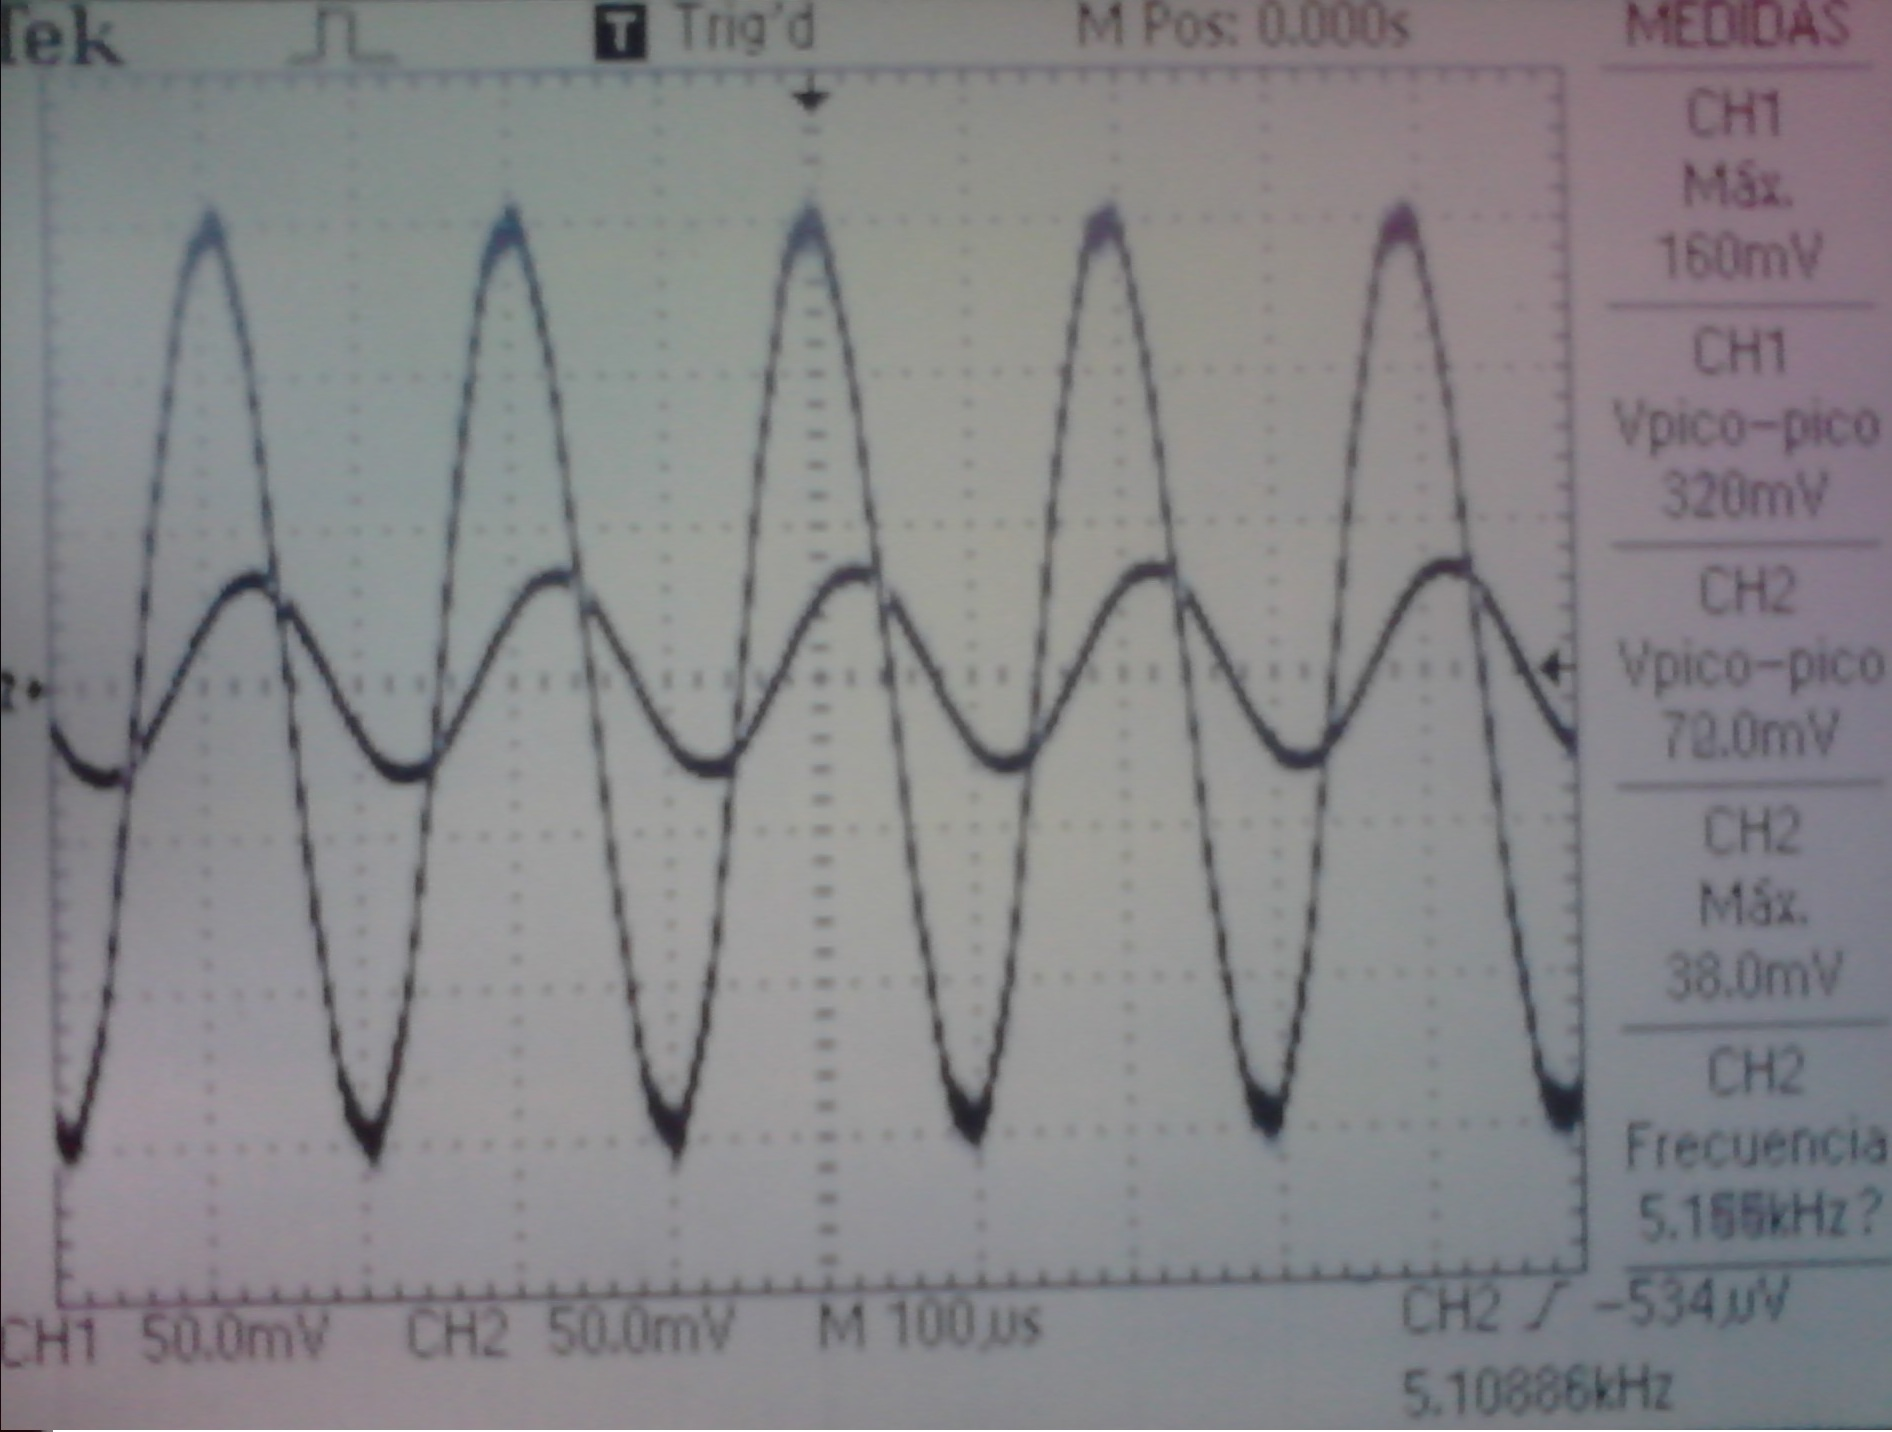
\includegraphics[scale=0.12]{mediciones/Ri_puntaX1.jpg}
\caption{Resultados obtenidos utilizando puntas X1}
\label{fig:medicion_Ri_X1}
\end{figure}

En la figura \ref{fig:medicion_Ri_X10} se muestran los resultados
obtenidos utilizando puntas de prueba X10.
Se calcula Ri:

\[ \displaystyle     R_i = \frac{1\,\unit{M\Omega}\  84.0\,\unit{mV}}{166\,\unit{mV} - 84.0\,\unit{mV}} 
\approx 1.02\,\unit{M\Omega}\]

Que es un valor similar al obtenido mediante calculos teóricos.
La punta de prueba X10 afecta menos a la medición ya que su modelo equivalente posee
una resistencia de $10\,\unit{M\Omega}$ en paralelo a un capacitor
de $20\,\unit{pF}$. El capacitor a una frecuencia de $5\,\unit{kHz}$ tiene una reactancia
de $10\,\unit{M\Omega}$, por lo que la punta X10 posee una reactancia equivalente
de $10\,\unit{M\Omega} // 10\,\unit{M\Omega} = 5\,\unit{M\Omega}$.
Esta resistencia en paralelo a $R_i$ afecta en menor medida a las mediciones,
ya que es mayor que $R_i$.

\begin{figure}[H]
\centering
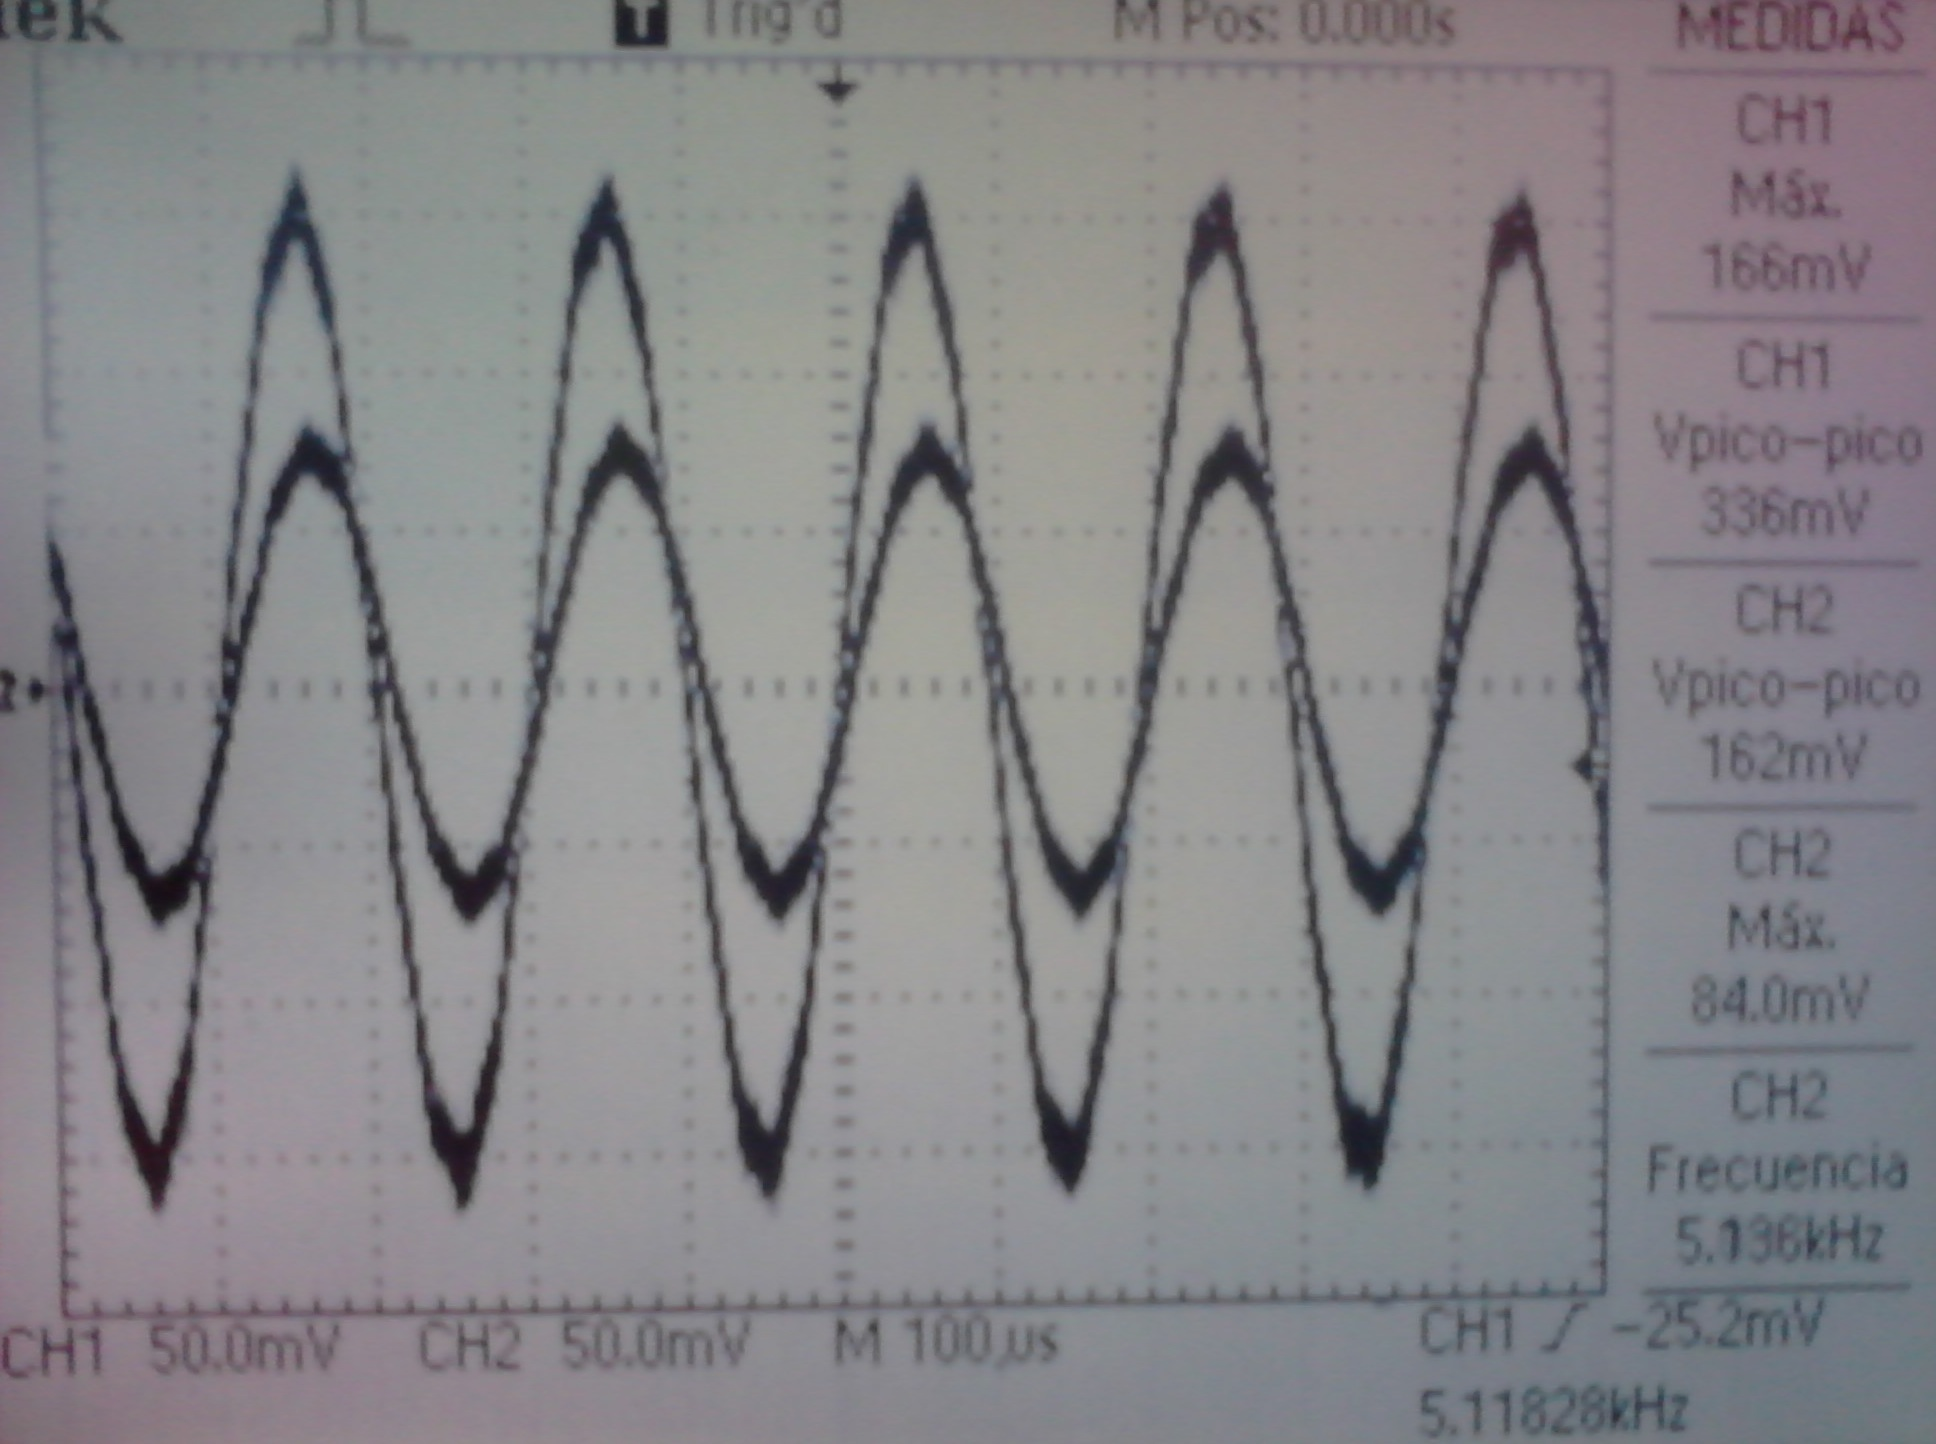
\includegraphics[scale=0.12]{mediciones/Ri_puntaX10.jpg}
\caption{Resultados obtenidos utilizando puntas X10}
\label{fig:medicion_Ri_X10}
\end{figure}

\subsubsection{Resistencia de salida \texorpdfstring{$R_o$}{TEXT}}

Utilizando el banco de medición de la figura \ref{fig:SIMURo_con_punta}
se obtuvo el resultado mostrado en la figura \ref{fig:medicion_Ro}.

Se obtiene la resistencia $R_{oL}$ mediante la ecuación \ref{eq:RoL},
utilizando los valores picos medidos.

\begin{equation}
    R_{oL} = \frac{R_p\ V_{CH1}}{V_{CH2} - V_{CH1}}
\label{eq:RoL}
\end{equation}

Reemplazando los valores obtenidos:

\[ \displaystyle R_{oL} = \frac{4.7\,\unit{k\Omega}\ 23.2\,\unit{mV}}{67.2\,\unit{mV} - 23.2\,\unit{mV}} 
= 2.5\,\unit{k\Omega} \]

Luego se despeja $R_o$ del paralelo $R_{oL} = R_L // R_o$.

\[ \displaystyle R_o = \frac{R_{oL}R_L}{R_L - R_{oL}}
= \frac{2.5\,\unit{k\Omega}\ 4.7\,\unit{k\Omega}}{4.7\,\unit{k\Omega} - 2.5\,\unit{k\Omega}} 
\approx 5.3\,\unit{k\Omega} \]

Que es un valor similar al obtenido mediante cálculos teóricos($4.7\,\unit{k\Omega}$).

\begin{figure}[H]
\centering
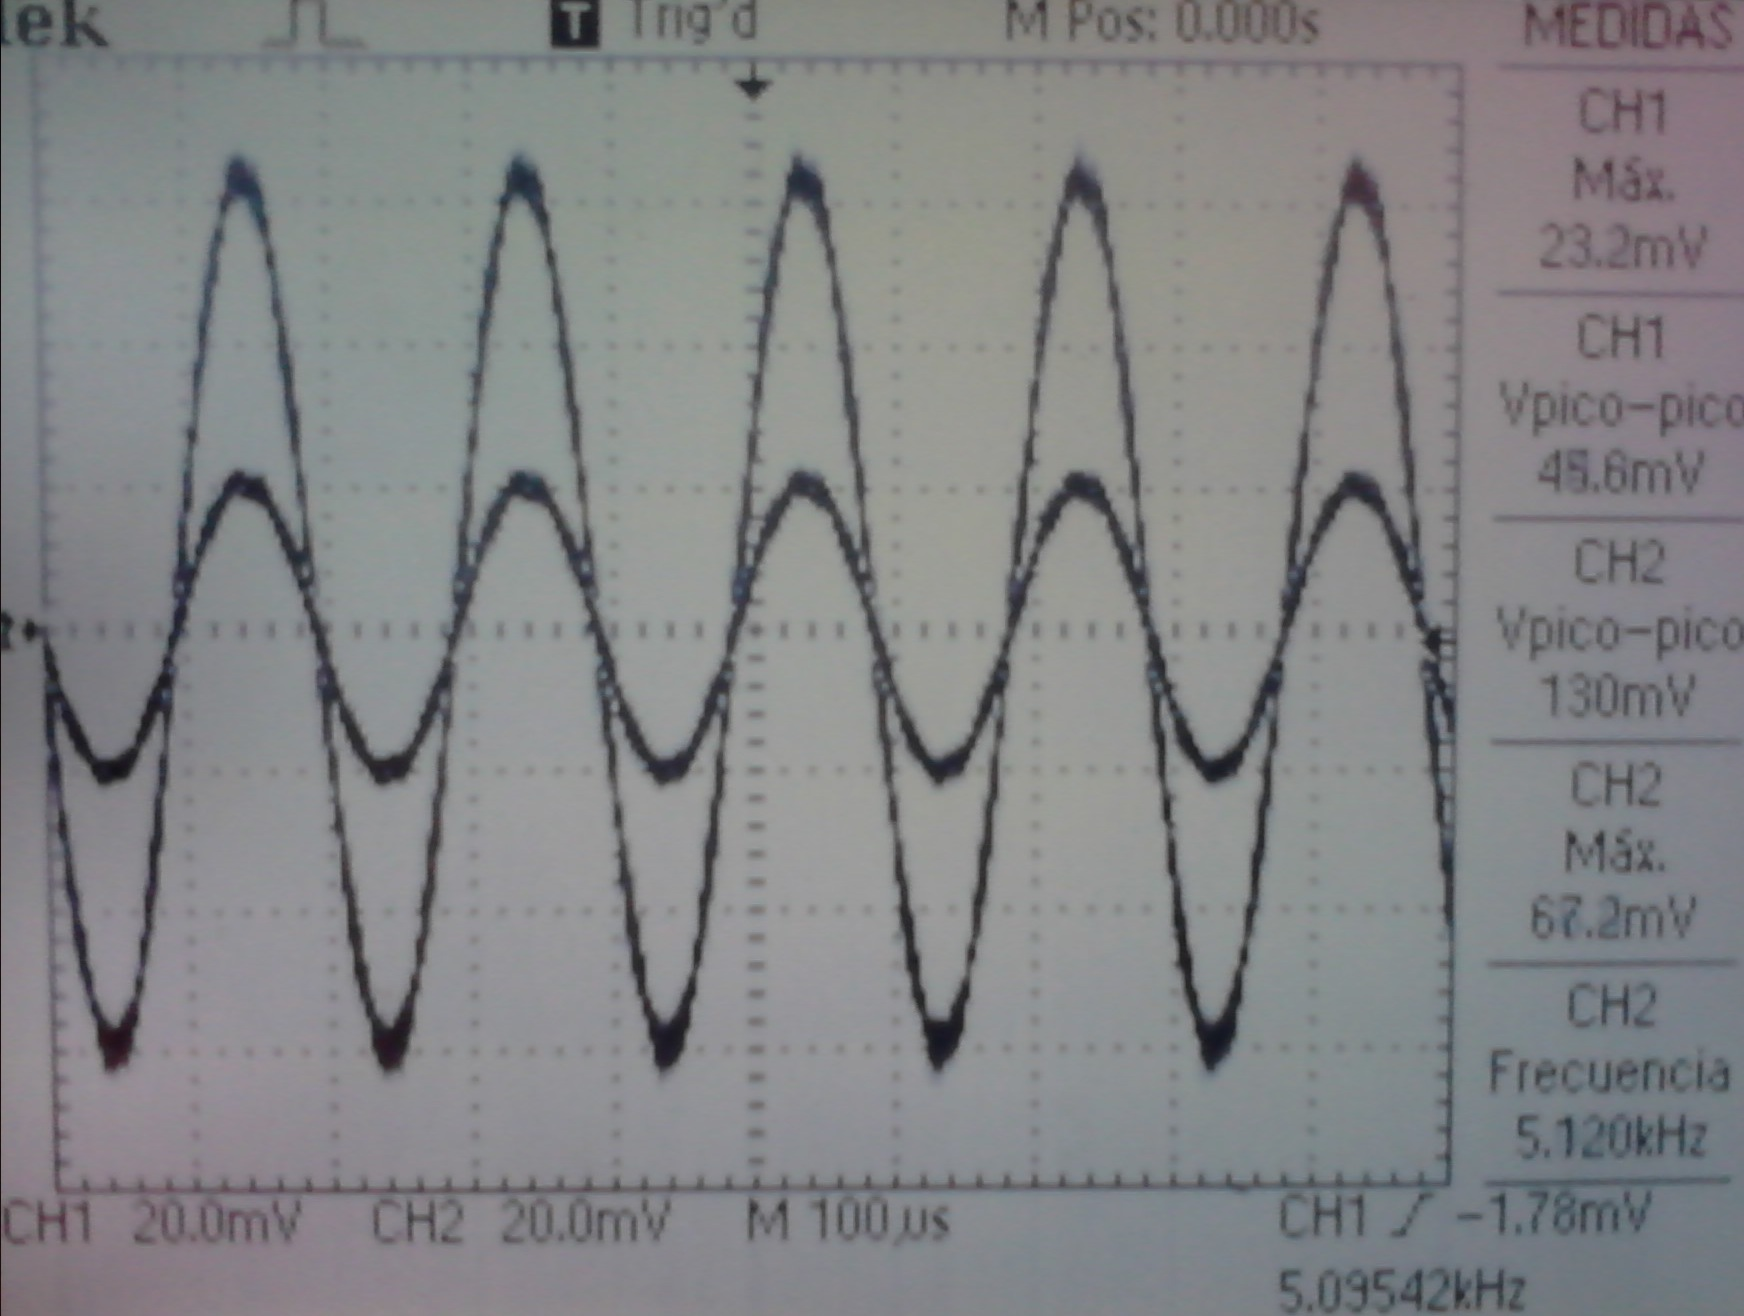
\includegraphics[scale=0.12]{mediciones/Ro_puntaX10.jpg}
\caption{Resultados obtenidos utilizando puntas X10}
\label{fig:medicion_Ro}
\end{figure}


\subsection{Excursión de salida}

\subsubsection{Excursión de salida sin distorsión}

En la medición de la excursión tuvimos en cuenta, como en el preinforme, la máxima amplitud de salida con baja distorsión ($\approx 15mV$ en la simulacion), además de la máxima excursión sin recorte y el $\widehat{V_{o_{max}}}$ para la señal ya recortada.

\begin{figure}[H]
\centering
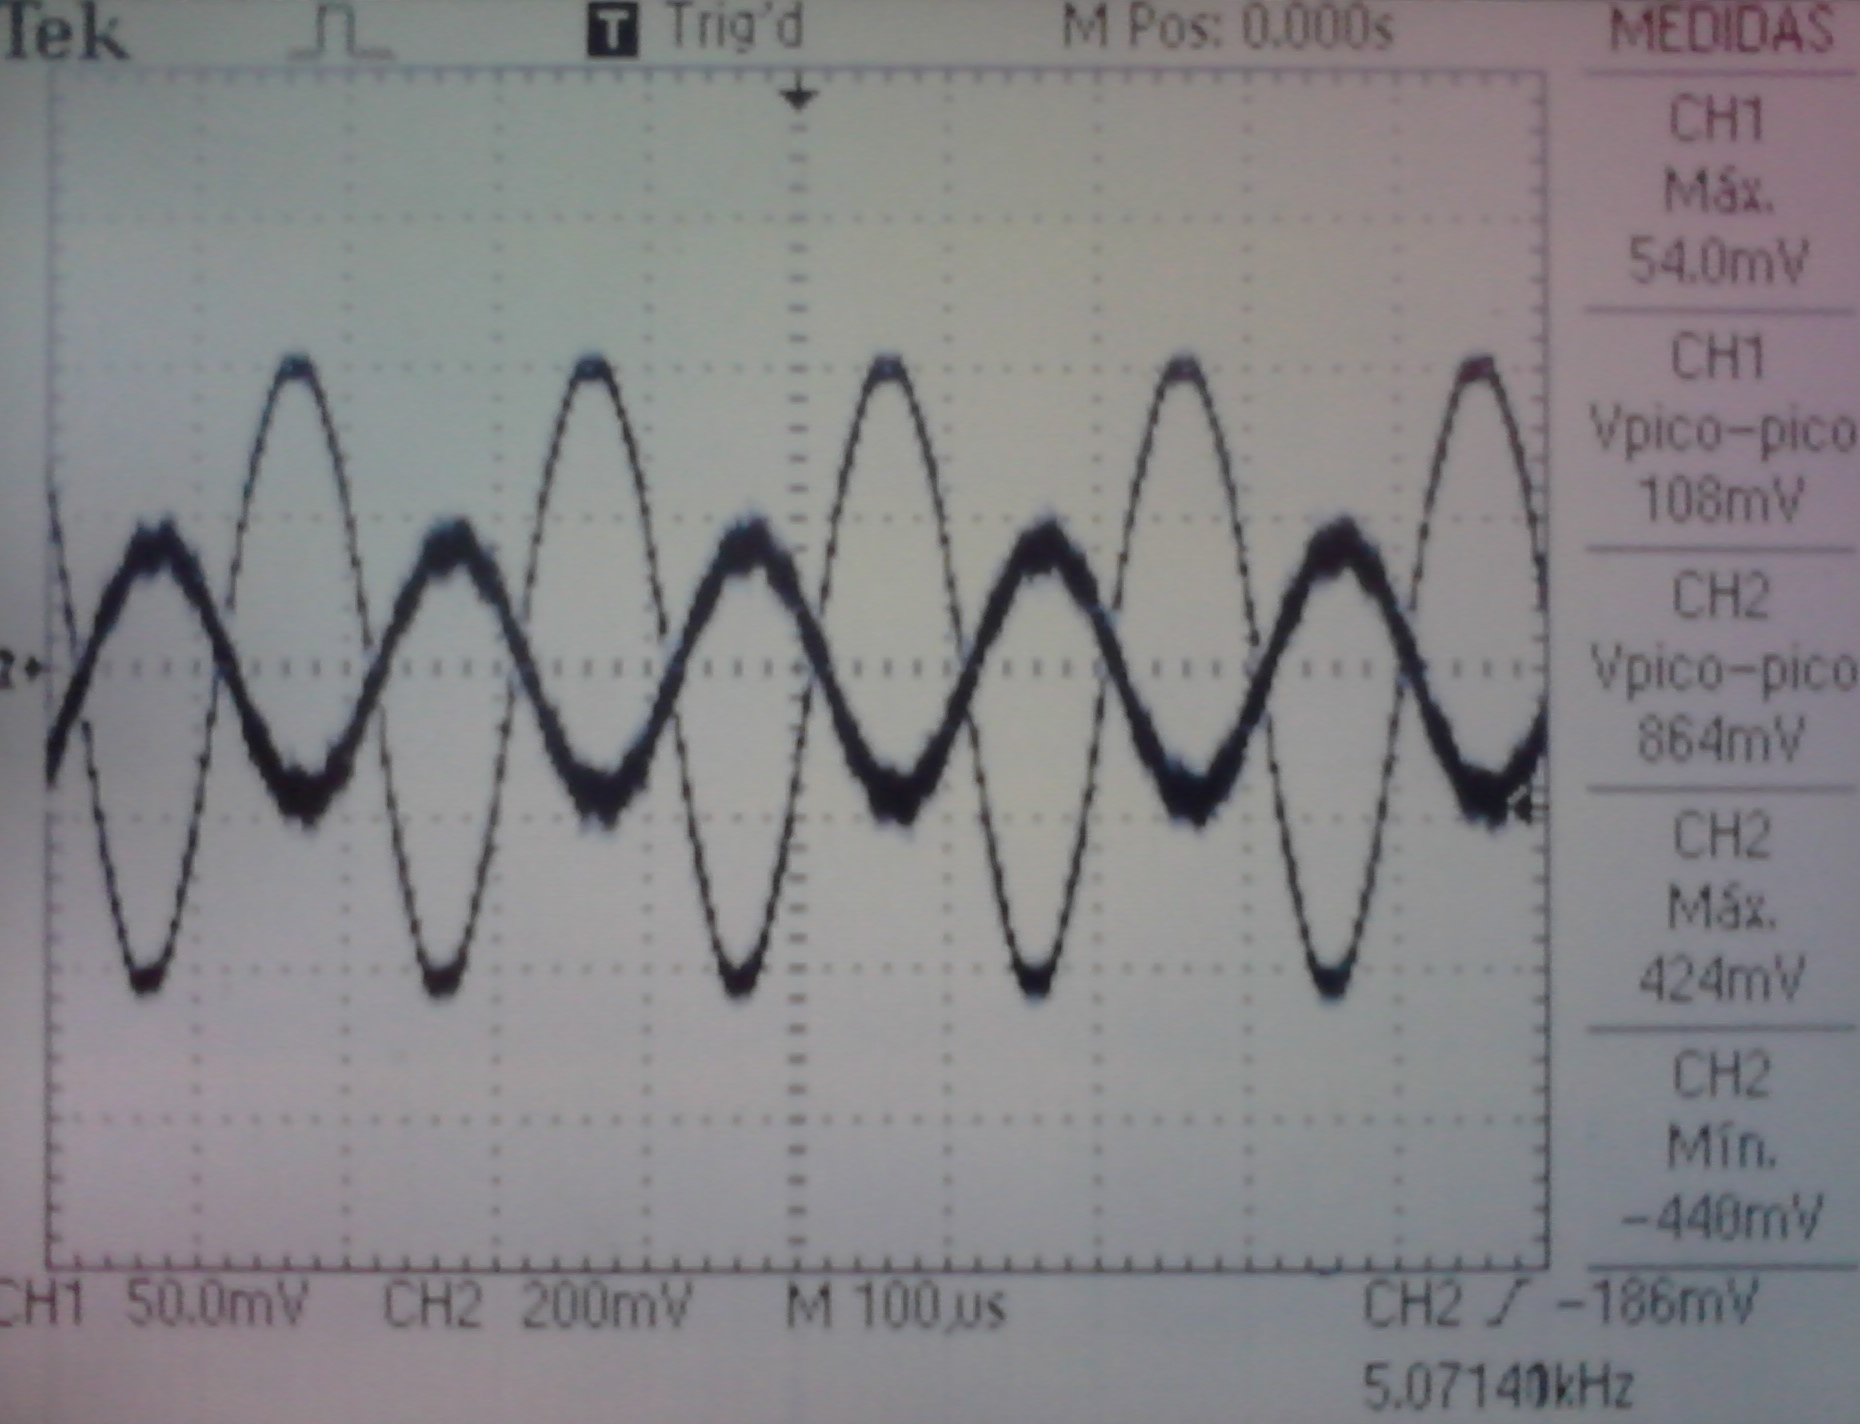
\includegraphics[scale=0.15]{mediciones/distorsion_54mV.jpg}
\caption{Distorsión. Señal de entrada y salida. $\widehat{V_{in}}=54mV$}
\label{fig:distorsion_54mV}
\end{figure}
La señal de entrada en este caso se fijó en un valor mayor a la simulación, ya que para menores amplitudes resultaban señales muy ruidosas y no se lograban visualizar bien en el osciloscopio. En la imagen se indican el máximo y mínimo para la señal de salida distorsionada.

Además, para la salida de la figura \ref{fig:distorsion_54mV}, se realizó la FFT desde el menú \textbf{Math} del osciloscopio. Y se obtuvo la imagen mostrada en la
figura \ref{fig:FFT_54mV}.

\begin{figure}[H]
\centering
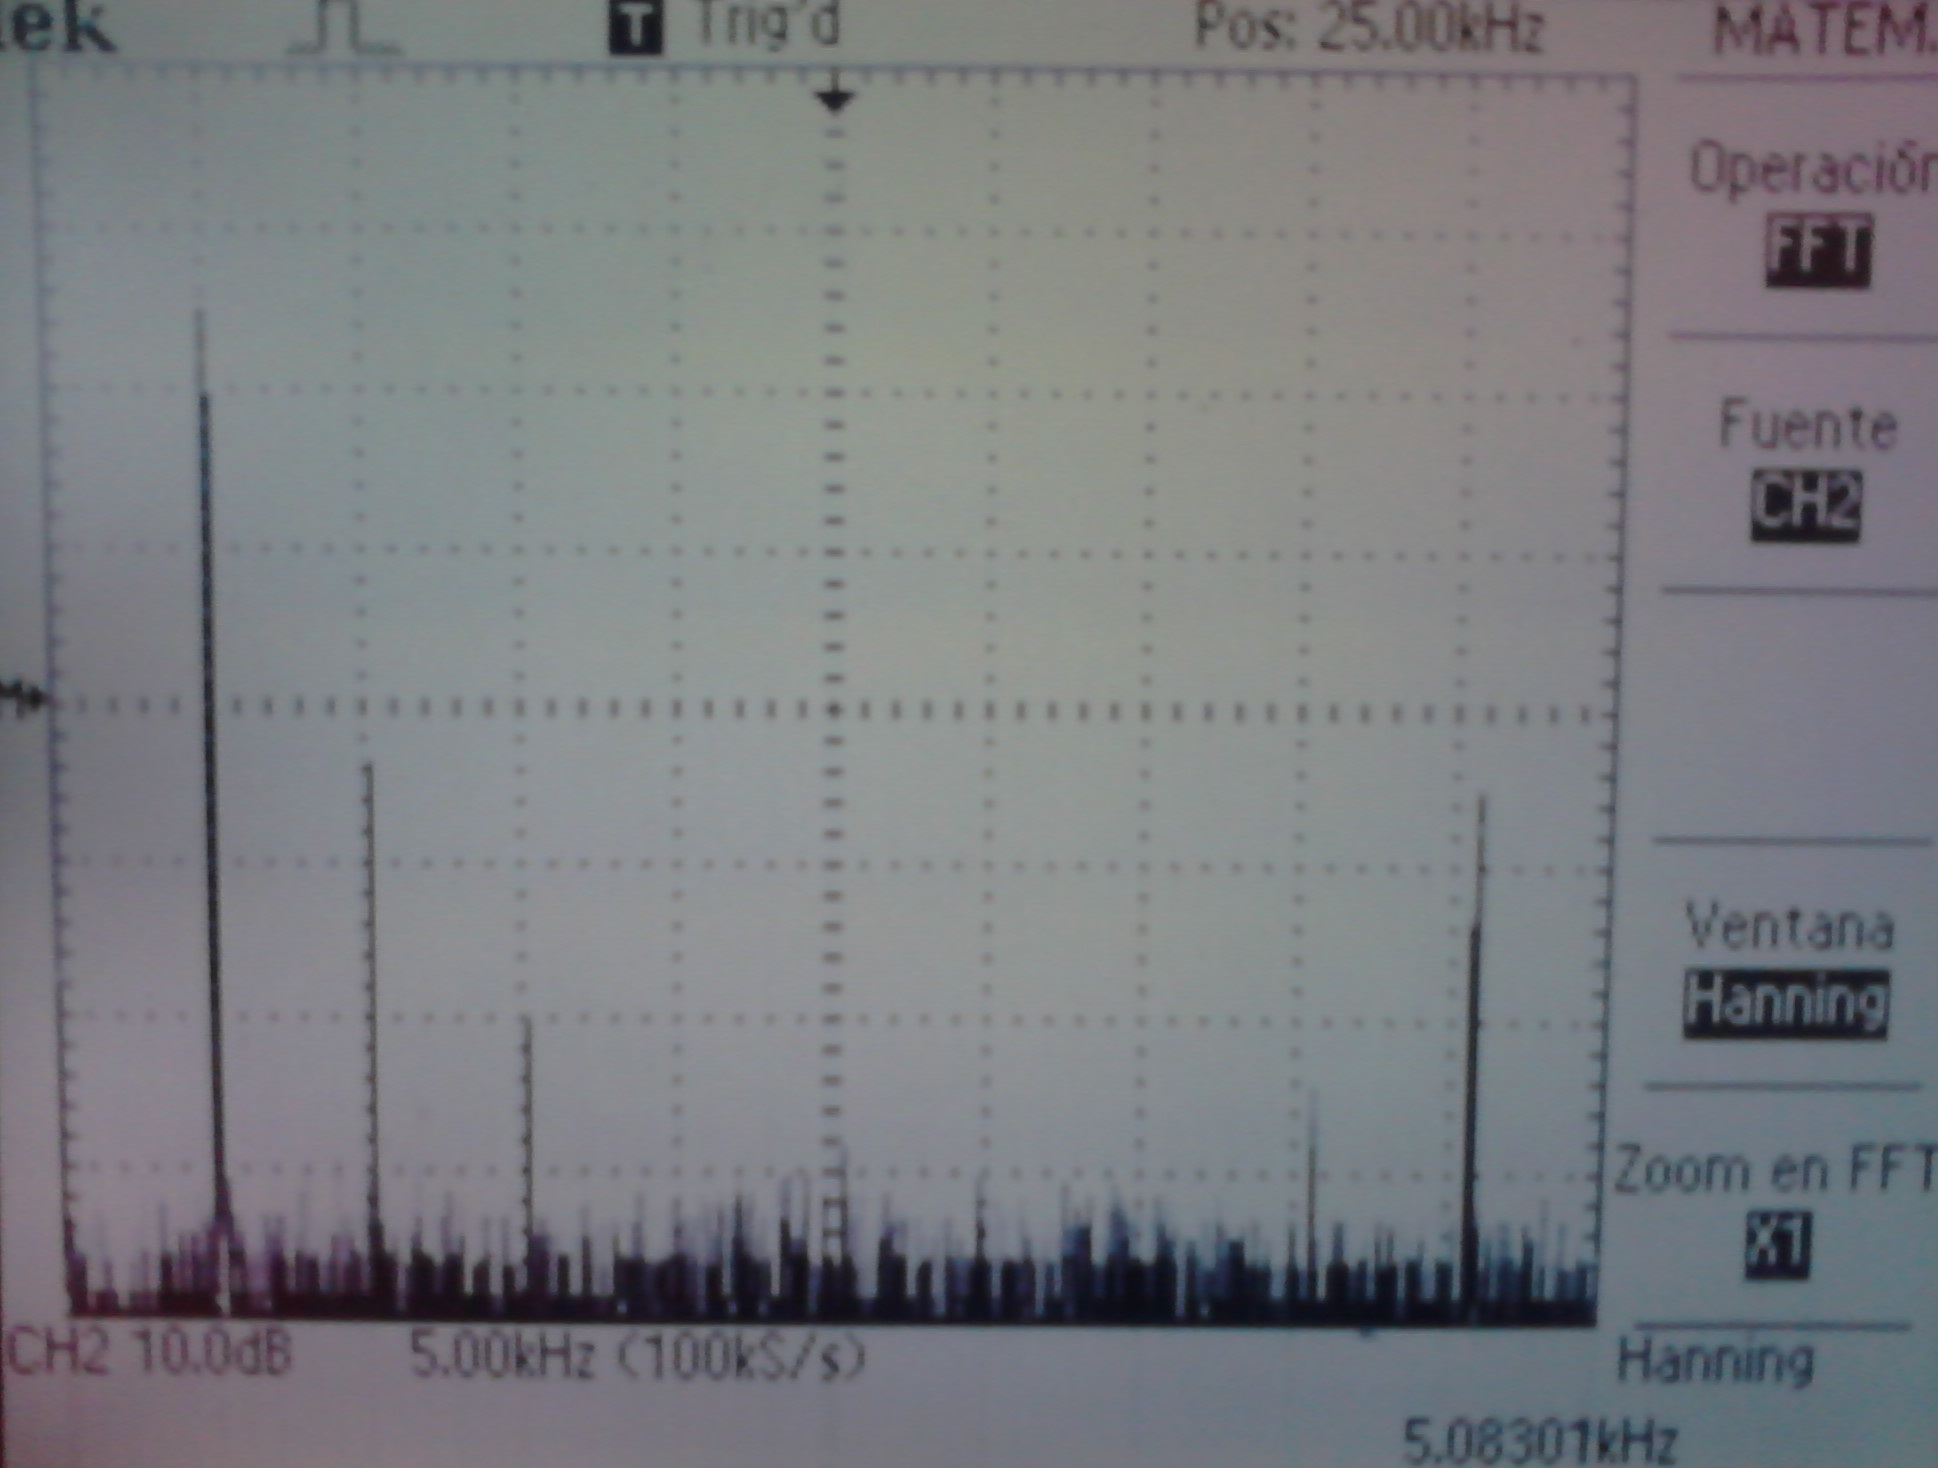
\includegraphics[scale=0.15]{mediciones/FFT_54mV.jpg}
\caption{Distorsión.FFT  osciloscopio para señal salida. $\widehat{V_{in}}=54\,\unit{mV}$}
\label{fig:FFT_54mV}
\end{figure}

A partir de esta captura se construye la tabla \ref{table:medicion_FFT} de valores normalizados (los más notables en la figura) para así obtener la distorsión armónica total.

Para obtener la amplitud normalizada, se despejó $\frac{Vi}{V_{ref}}$
de la ecuación \ref{eq:ecuacion_dB}.

\begin{equation}
dB_i = 20\,\unit{dB}\ log\left(\frac{V_i}{V_{ref}}\right)
\label{eq:ecuacion_dB}
\end{equation}

Despejando se obtiene la ecuación \ref{eq:ecuacion_norm_dB}.

\begin{equation}
\frac{V_i}{V_{ref}} = 10^{\frac{dB_i}{20\,\unit{dB}}}
\label{eq:ecuacion_norm_dB}
\end{equation}


\begin{table}[H]
\centering
\begin{tabular}{|c|c|c|c|c|c|} 
\hline
Frecuencia & $5\,\unit{kHz}$ & $10\,\unit{kHz}$ & $15\,\unit{kHz}$ & $40\,\unit{kHz}$ & $45\,\unit{kHz}$ \\ \hline
Amplitud en dB & $65\,\unit{dB}$ & $36\,\unit{dB}$ & $20\,\unit{dB}$ & $16\,\unit{dB}$ & $35\,\unit{dB}$ \\ \hline
Amplitud normalizada & $1778$ & $63$ & $10$ & $6.3$ & $56$ \\ \hline
\end{tabular}
\caption{Datos extraídos de la función FFT del osciloscopio.}
\label{table:medicion_FFT}
\end{table}


Finalmente se obtiene la distorsión armónica total mediante la ecuación
\ref{eq:distorsion_armonica_total}. Siendo $V_{fundamental}$ la amplitud
obtenida para la frecuencia del generador de señales, $5\,\unit{kHz}$.

\begin{equation}
THD = \frac{\sum\limits_{i=2}^{n} V_i}{V_{fundamental}}
\label{eq:distorsion_armonica_total}
\end{equation}

Se obteniendose:

\[ \displaystyle THD = \frac{63+10+6.3+56}{1778} \approx 0.076 = 7.6\,\unit{\%} \]

\subsubsection{Excursión de salida sin recorte}

La máxima excursión sin recorte obtenida fue para un $\widehat{V_{in}}=224\,\unit{mV}$, además para verificar el valor máximo en el que recortaba la salida se obtuvo una captura de la pantalla para una amplitud de entrada aún mayor. El valor medido en este caso resultó $\widehat{V_{o_{max}}}=1.48\,\unit{V}$. Es lógico que resulte un poco menor a las simulaciones ya que la amplificación medida resultó menor.
A continuación las imágenes correspondientes.

\begin{figure}[H]
\centering
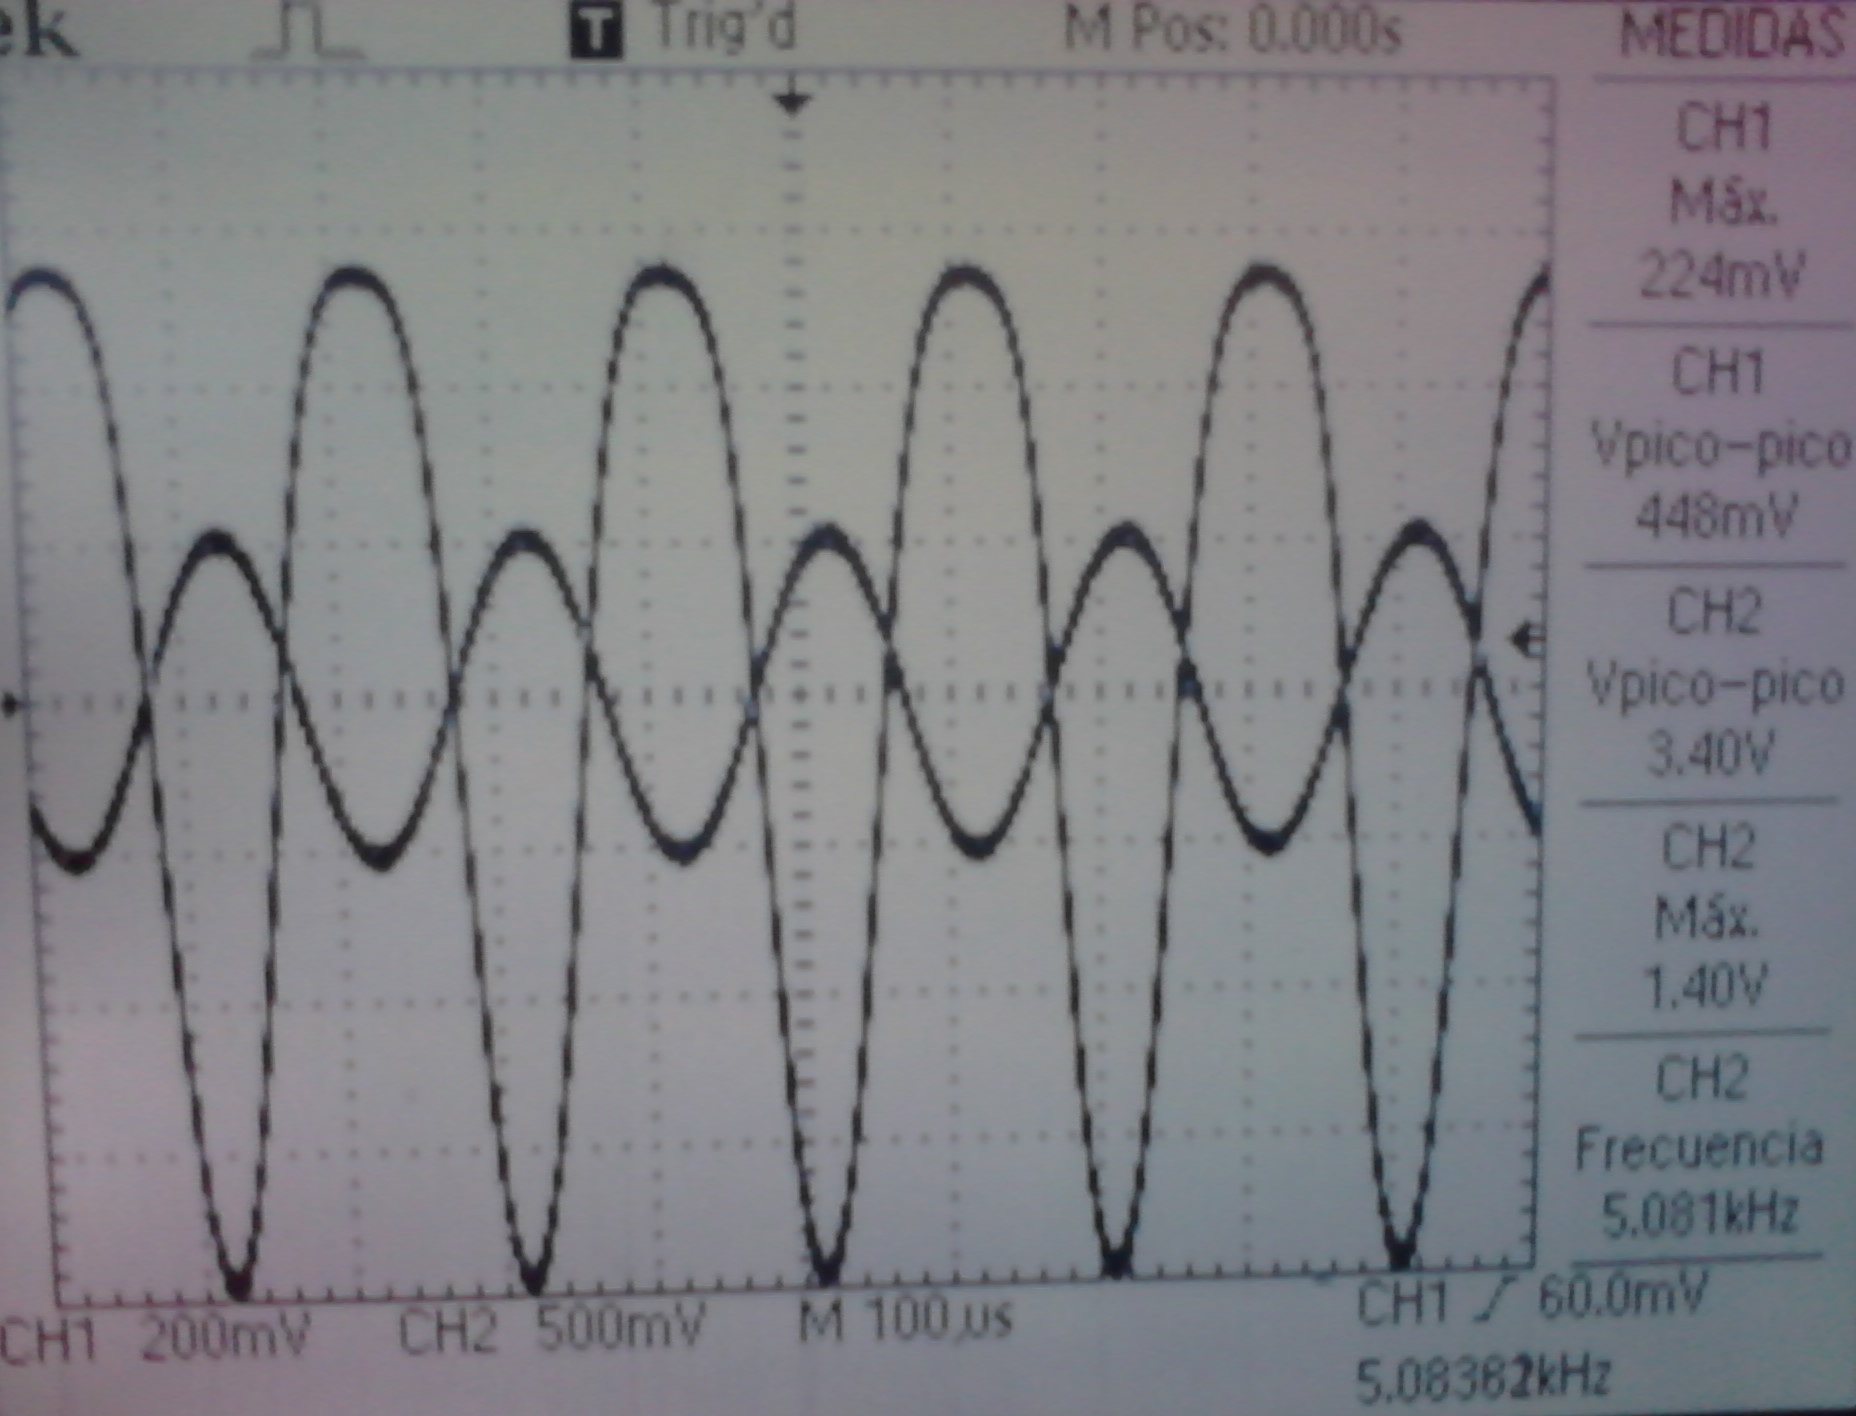
\includegraphics[scale=0.15]{mediciones/Recorte_224mV.jpg}
\caption{Señal de entrada y salida para máxima excursión sin recorte. $\widehat{V_{in}}=224\,\unit{mV}$}
\label{fig:Recorte_224mV}
\end{figure}

\begin{figure}[H]
\centering
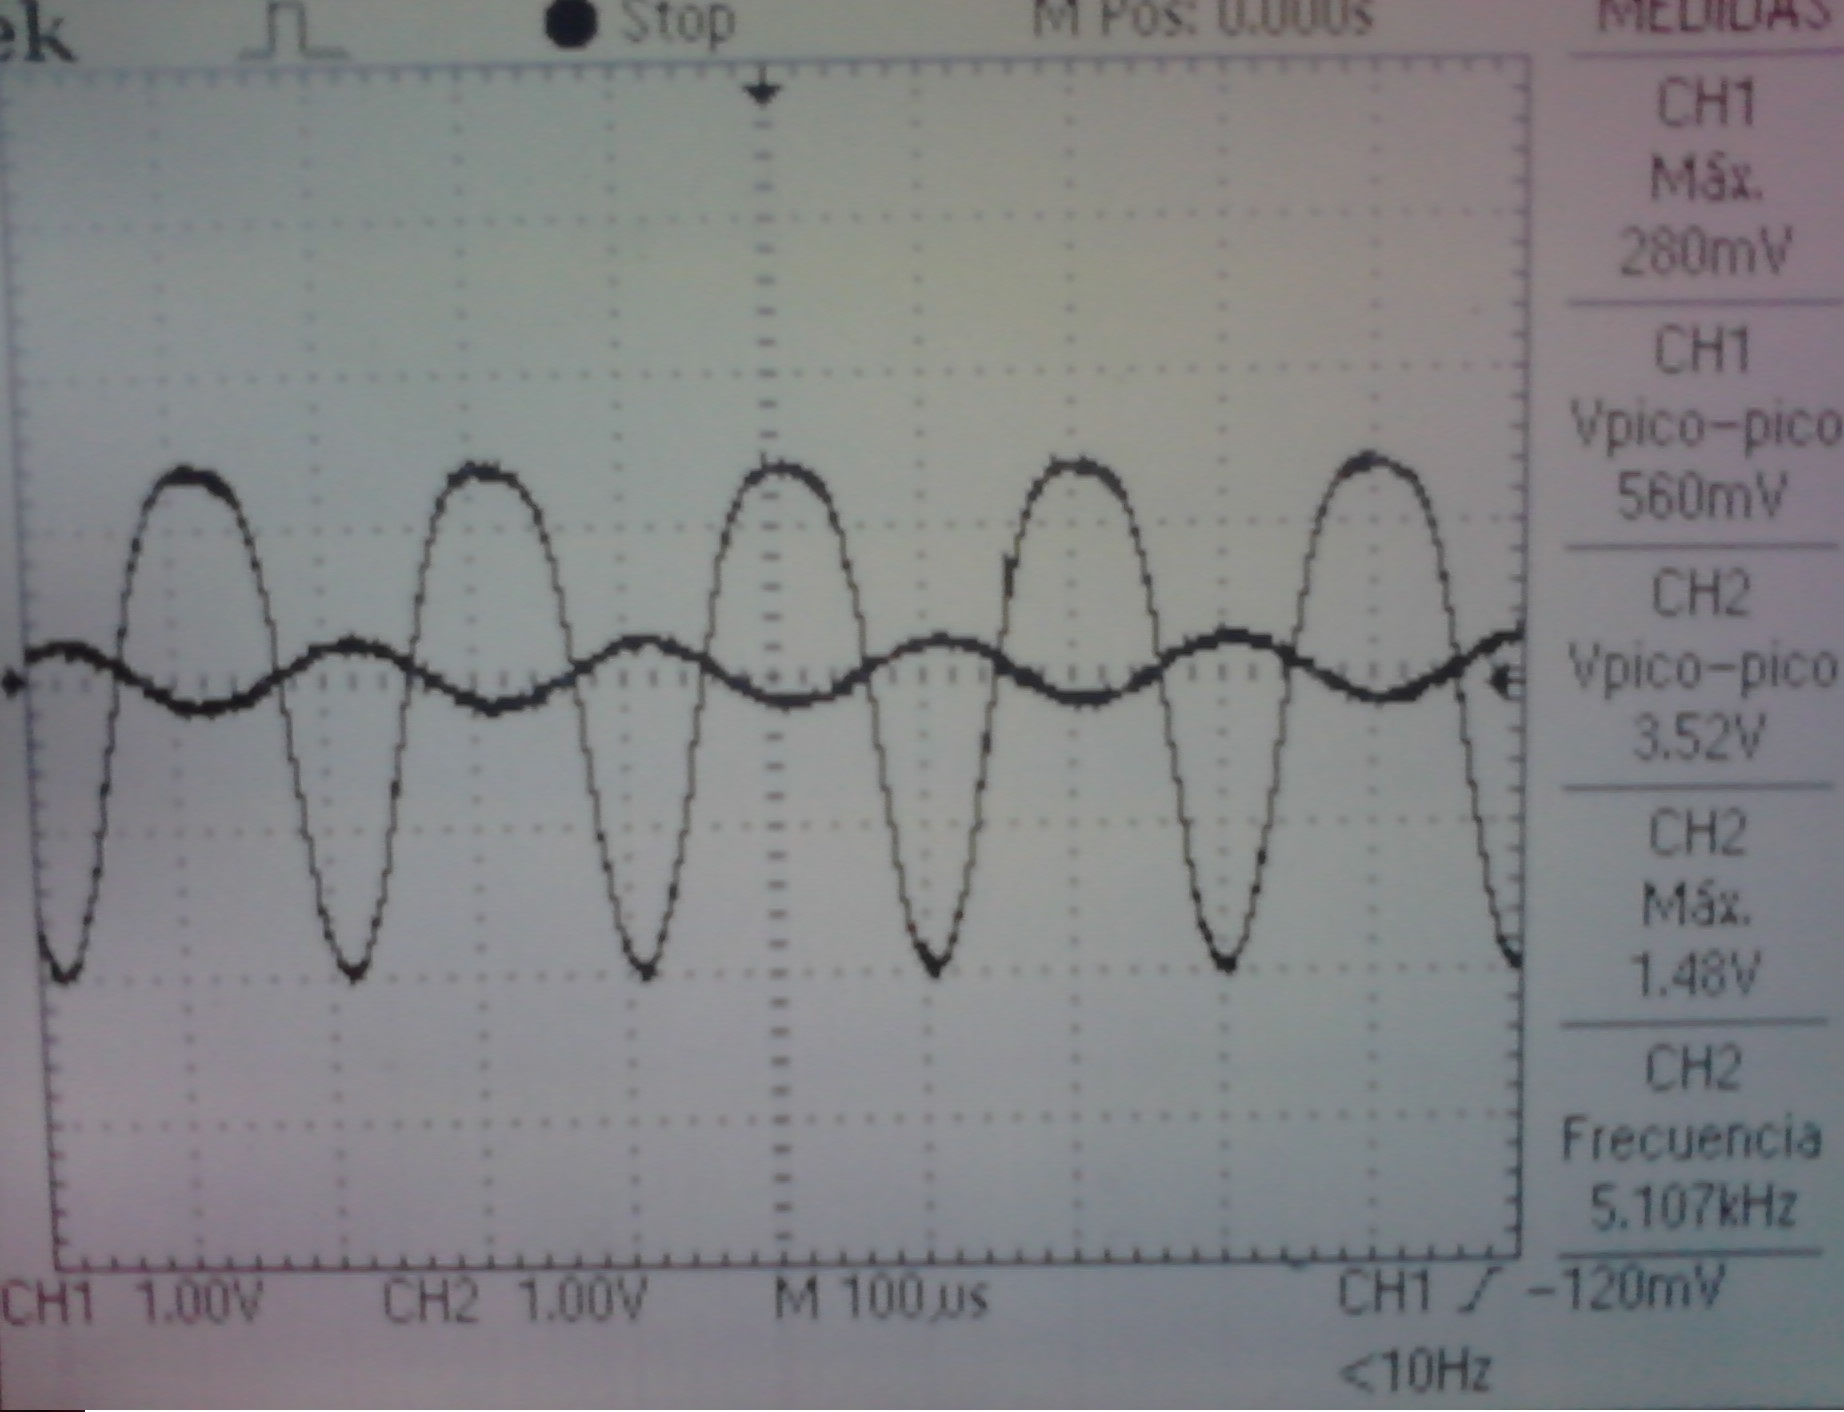
\includegraphics[scale=0.15]{mediciones/Recorte_280mV.jpg}
\caption{Señal de entrada y salida. $\widehat{V_{o_{max}}}=1.48\,\unit{V}$. $\widehat{V_{in}}=280mV$}
\label{fig:Recorte_280mV}
\end{figure}


\subsection{Respuesta en frecuencia para \texorpdfstring{$A_{vs}$}{TEXT}}

\subsubsection{Análisis en bajas frecuencias}

Se utilizó el banco de medición mostrado en la figura
\ref{fig:SIMUreposo} utilizando puntas de prueba X10.
Se midió la señal de salida y de entrada, para un rango
de frecuencias de $400\,\unit{Hz}$ a $9\,\unit{kHz}$.

En la figura \ref{fig:medicion_bajas_frecuencias} se muestra
la curva obtenida en escala logarítmica, marcando con una
linea roja la amplificación que esta a $-3\,\unit{dB}$ de
la amplificación a frecuencias medias.
Obteniéndose aproximadamente la frecuencia de corte
inferior $f_l = 1.25\,\unit{kHz}$.

\begin{figure}[H]
\centering
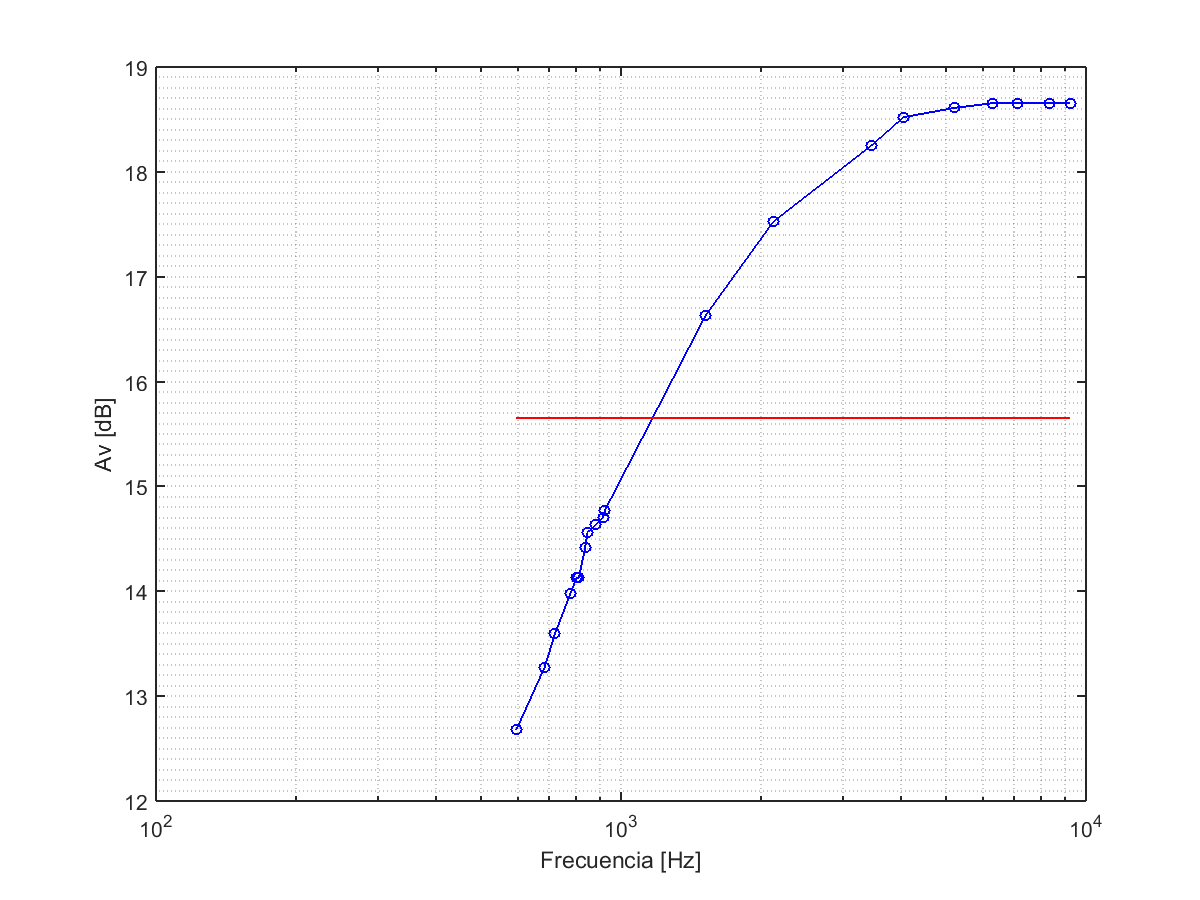
\includegraphics[scale=0.6]{mediciones/bajas_frecuencias.png}
\caption{Amplificación obtenida para un barrido en bajas frecuencias.}
\label{fig:medicion_bajas_frecuencias}
\end{figure}

\subsubsection{Análisis en altas frecuencias}

Luego se realizó un barrido en frecuencias desde los $100\,\unit{kHz}$ hasta los
$10\,\unit{MHz}$. Luego se armó una curva con los datos obtenidos y en cada
grafico se trazó una recta de color rojo para indicar
los $-3\,\unit{dB}$ respecto del $A_v$ en frecuencias medias.

En la figura \ref{fig:alta_frec_puntaX10} se muestra la curva obtenida utilizando
una punta de prueba X10 en la salida. Se obtuvo aproximadamente una frecuencia de corte
$f_l = 3.1\,\unit{MHz}$. Que es un valor similar al simulado.

En la figura \ref{fig:alta_frec_punta_activa} se muestra la curva obtenida utilizando
una punta de prueba activa en la salida. Se obtuvo aproximadamente una frecuencia de corte
$f_l = 7.0\,\unit{MHz}$. Este valor dista bastante del simulado.

\begin{figure}[H]
\centering
\begin{subfigure}{.5\textwidth}
  \centering
  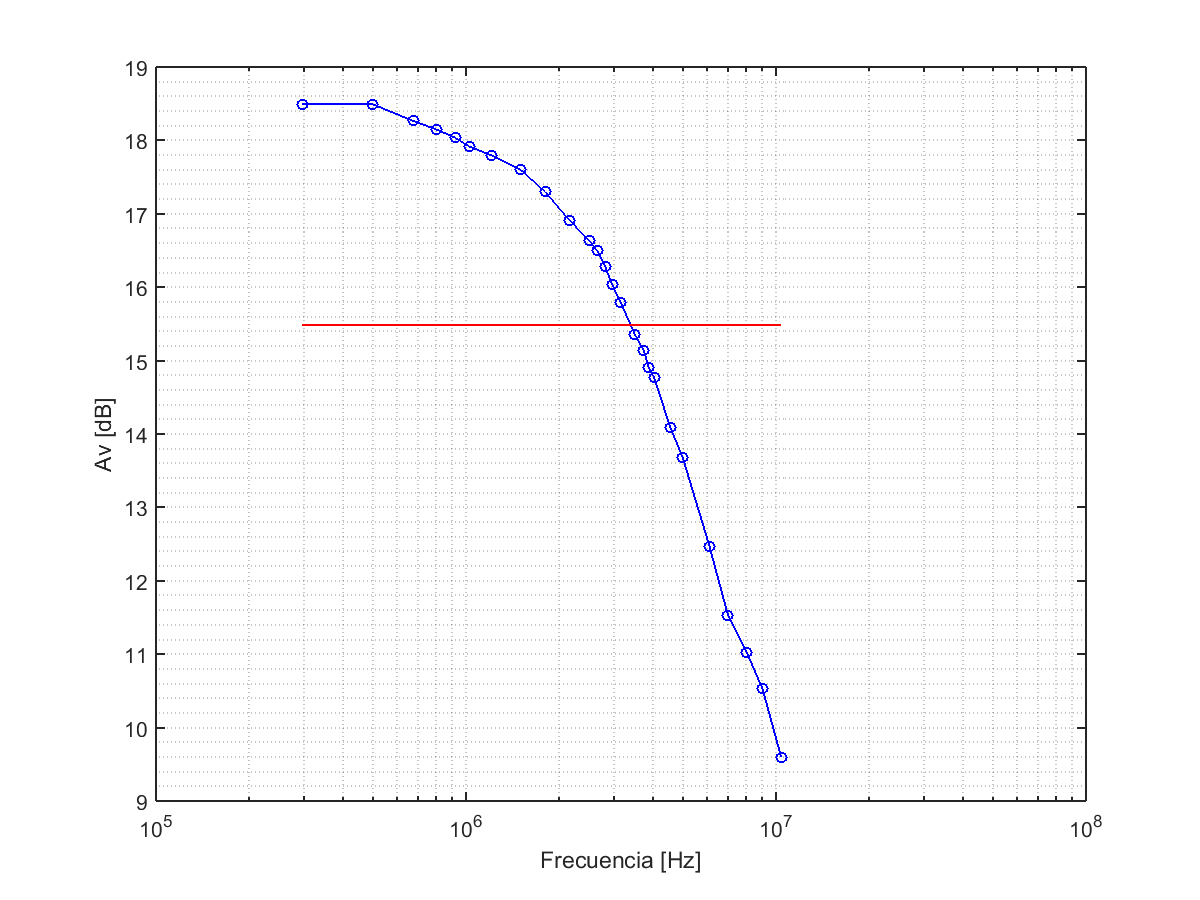
\includegraphics[width=1\linewidth]{mediciones/altas_frecuencias_PuntaX10.png}
  \caption{Altas frecuencias utilizando punta X10}
  \label{fig:alta_frec_puntaX10}
\end{subfigure}%
\begin{subfigure}{.5\textwidth}
  \centering
  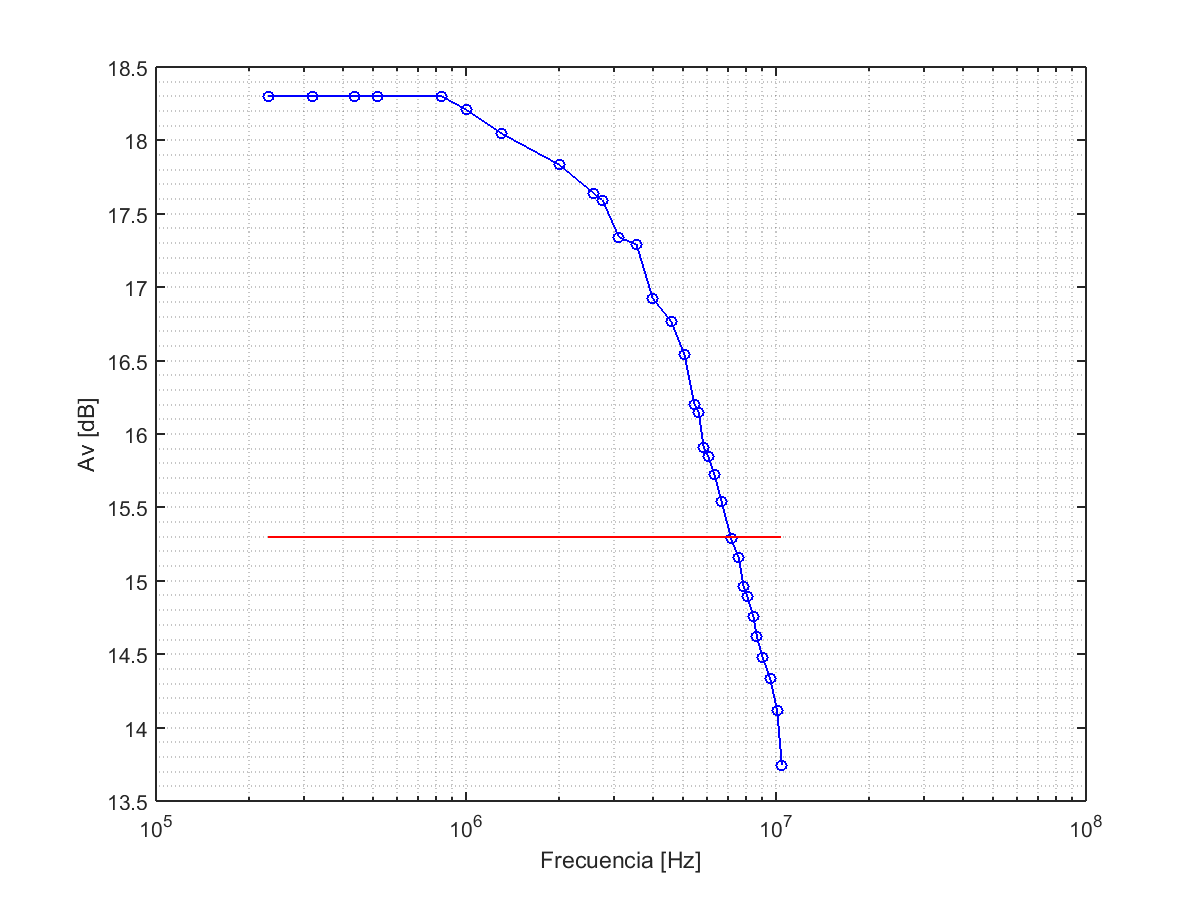
\includegraphics[width=1\linewidth]{mediciones/altas_frecuencias_PuntaActiva.png}
  \caption{Altas frecuencias utilizando punta activa}
  \label{fig:alta_frec_punta_activa}
\end{subfigure}
\caption{Amplificación obtenida para un barrido en altas frecuencias.}
\label{fig:medicion_alta_frec}
\end{figure}

\section{Comparación de resultados}

\subsection{Punto de reposo}
La diferencia entre los valores calculados analíticamente (tabla \ref{table:valoresreposo}) y los valores simulados (tabla \ref{table:valoresreposoSIMU}), difieren de los medidos (tabla \ref{table:valoresreposomedidos}) debido a que los cálculos teóricos y posterior simulación fueron hechos en base a un modelo, que se aproxima a la realidad pero no es exacto


\subsection{Amplificación de tensión total (\texorpdfstring{$A_v$}{TEXT}) a frecuencias medias}

En la tabla \ref{table:compganancias} pueden observarse las ganancias obtenidas para cada método, y en la tabla \ref{table:compgananciaserror} los errores respecto a la medición.

\begin{table}[H]
\centering
\begin{tabular}{|c|c|c|} 
\hline
Método & $A_{v}$  \\ \hline
Analítico & -10.8 \\ \hline
Simulación & -10 \\ \hline
Medición & -6.78\\ \hline
\end{tabular}
\caption{Tabla comparativa de las ganancias obtenidas mediante distintos métodos}
\label{table:compganancias}
\end{table}

\begin{table}[H]
\centering
\begin{tabular}{|c|c|c|} 
\hline
Método & Error \\ \hline
Analítico & 59.2 \%  \\ \hline
Simulación &  47.3 \% \\ \hline
\end{tabular}
\caption{Tabla con los errores respecto a la medición}
\label{table:compgananciaserror}
\end{table}

Si bien entre el valor de la ganancia calculado analíticamente y mediante simulación no hay gran diferencia, ambos son muy distintos respecto al valor medido. Esto se debe a que la corriente y tensiones de reposo son muy parecidas en la simulación y el cálculo analítico, pero difieren mucho de lo medido, por lo que al cambiar el punto de operación, también se modifica la ganancia.


\subsection{Resistencia de entrada y salida}
Como ya se explicó anteriormente, las mayores diferencias entre los resultados teóricos y simulaciones con respecto a las mediciones ocurrieron en el caso de la utilización de la punta X1, ya que la influencia de su reactancia interna alteró significativamente el resultado obtenido.

\begin{table}[H]
\centering
\begin{tabular}{|c|c|c|c|} 
\hline
Método & $R_i$ &$R_o$ \\ \hline
Analítico & $1\,\unit{M\Omega}$ & $4,7\,\unit{k\Omega}$ \\ \hline
Simulación punta x10 & $910\,\unit{k\Omega}$ & $4,7\,\unit{k\Omega}$ \\ \hline
Medición punta x1 & $333\,\unit{k\Omega}$ & - \\ \hline
Medición punta x10 & $1,02\,\unit{M\Omega}$ & $5,3\,\unit{k\Omega}$ \\ \hline % el \, te agrega un medio espacio entre el numero y las unidades
%que flashero ver como escribis jajaj el error es pq el 'it no habia que poner los numeros esos en math mode, osea entre $ $ para que no tire error
\end{tabular}
\caption{Tabla comparativa de resultados para $R_i$ y $R_o$}
\label{table:compResistencias}
\end{table}

\subsection{Excursión de salida}

En la tabla \ref{table:compexcursion} se muestran las máximas excursiones obtenidas mediante
distintos métodos. La tensión de salida sin recorte son similares para todos los métodos, pero
esto no ocurre con la tensión máxima sin distorsión. Esto se debe a que se tomó como criterio
para cumplir con la inecuación \ref{eq:distorsion} que $\Delta V_{GS}$ sea 10 veces
mas chico que $\frac{V_{GSQ}-V_T}{2}$ de forma arbitraria. Por los resultados obtenidos
en las mediciones se podría haber tomado una cota mayor.

\begin{table}[H]
\centering
\begin{tabular}{|c|c|c|c|c|} 
\hline
Método & máx excursión s/recorte & $V_{in_{max}}$ s/distorsión &distorsión &$V_{out_{max}}$ recorte\\ \hline
Analítico & 1.65V &14,8mV& - &1.65V \\ \hline
Simulación & 1,6V&15mV &1,20&1,6V \\ \hline
Medición &1.4V  &54 mV & &1.48V\\ \hline
\end{tabular}
\caption{Tabla comparativa para resultados de excursión de salida}
\label{table:compexcursion}
\end{table}

\subsection{Respuesta en frecuencia para \texorpdfstring{$A_{vs}$}{TEXT}}
\begin{table}[H]
\centering
\begin{tabular}{|c|c|c|} 
\hline
Método & $f_l$&$f_h$ \\ \hline
Analítico & 894Hz & 78,8 MHz\\ \hline
Analítico punta x10 & - & 3,12MHz\\ \hline
Analítico punta activa& -  &35,5MHz \\ \hline
Simulación & 880Hz&80,7MHz \\ \hline
Simulación punta x10& 880Hz& 3,3MHz\\ \hline
Simulación punta activa&  880Hz&52MHz \\ \hline
Medición punta x10&1,25kHz &3,1MHz\\ \hline
Medición punta activa&- &7,0MHz\\ \hline
\end{tabular}
\caption{Tabla comparativa de resultados de respuesta en frecuencia para $A_{vs}$}
\label{table:compfrecuencias}
\end{table}

Se puede ver que la $f_h$ hallada para la medición con punta activa difiere considerablemente de la
simulada, esto puede deberse a que el modelo utilizado para dicha punta en la simulación 
dista bastante del equivalente real. Esto es, dado que se consideran capacitancias muy chicas (del
orden de los pF), las mediciones se ven afectadas por las distintas capacitancias parásitas presentes en el banco de medición(cable coaxial, PCB).

\section{Conclusión}

El punto de reposo difirió de lo calculado y simulado. Ya que en las mediciones
este depende de parámetros de fabricación que son difíciles de regular.

Es necesario tener en cuenta como afectan los instrumentos de medición al circuito.
Para la resistencia de entrada el resultado difiere mucho en base a la punta utilizada.
Ya que la impedancia de entrada de la punta era comparable con la resistencia a medir.

Lo mismo ocurrió para la medición de la frecuencia de corte superior ya que  el capacitor de la
punta de prueba X10 afectó considerablemente a la frecuencia de corte medida. Esto
se pudo corregir utilizando una punta de prueba activa, a pesar de que el resultado obtenido
difirió del simulado y calculado ya que el modelo de la punta de prueba activa
difiere del real, y en los cálculos y simulaciones no se tuvo en cuenta las capacitancias
parásitas de los cables coaxial y del circuito.

El criterio tomado para disminuir la distorsión en la señal de salida fue muy riguroso.
Ya que se decidió tomar que $\Delta V_{GS}$ sea 10 veces menor que $\frac{V_{GSQ}-V_T}{2}$.
Quedando limitado el circuito a señales de entrada de amplitud muy chicas. 

\end{document}